\documentclass{book}
\usepackage{fancyvrb}
\usepackage{color}
\usepackage[utf8]{inputenc}
\usepackage[a4paper, total={6.2in, 9in}]{geometry}
\usepackage[many]{tcolorbox}
\usepackage[T1]{fontenc}
\usepackage[slovene]{babel}

\usetikzlibrary{calc}

\setlength\parindent{0pt}

\makeatletter
\def\PY@reset{\let\PY@it=\relax \let\PY@bf=\relax%
    \let\PY@ul=\relax \let\PY@tc=\relax%
    \let\PY@bc=\relax \let\PY@ff=\relax}
\def\PY@tok#1{\csname PY@tok@#1\endcsname}
\def\PY@toks#1+{\ifx\relax#1\empty\else%
    \PY@tok{#1}\expandafter\PY@toks\fi}
\def\PY@do#1{\PY@bc{\PY@tc{\PY@ul{%
    \PY@it{\PY@bf{\PY@ff{#1}}}}}}}
\def\PY#1#2{\PY@reset\PY@toks#1+\relax+\PY@do{#2}}

\@namedef{PY@tok@c}{\def\PY@tc##1{\textcolor[rgb]{0.63,0.63,0.88}{##1}}}
\@namedef{PY@tok@cp}{\def\PY@tc##1{\textcolor[rgb]{0.19,0.51,0.25}{##1}}}
\@namedef{PY@tok@k}{\let\PY@bf=\textbf\def\PY@tc##1{\textcolor[rgb]{0.00,0.00,0.67}{##1}}}
\@namedef{PY@tok@o}{\def\PY@tc##1{\textcolor[rgb]{1.00,0.02,0.02}{##1}}}
\@namedef{PY@tok@p}{\def\PY@tc##1{\textcolor[rgb]{1.00,0.02,0.02}{##1}}}
\@namedef{PY@tok@n}{\def\PY@tc##1{\textcolor[rgb]{0.05,0.05,0.05}{##1}}}
\@namedef{PY@tok@s}{\def\PY@tc##1{\textcolor[rgb]{0.16,0.16,1.00}{##1}}}
\@namedef{PY@tok@m}{\def\PY@tc##1{\textcolor[rgb]{0.94,0.03,0.94}{##1}}}
\@namedef{PY@tok@kc}{\let\PY@bf=\textbf\def\PY@tc##1{\textcolor[rgb]{0.00,0.00,0.67}{##1}}}
\@namedef{PY@tok@kd}{\let\PY@bf=\textbf\def\PY@tc##1{\textcolor[rgb]{0.00,0.00,0.67}{##1}}}
\@namedef{PY@tok@kn}{\let\PY@bf=\textbf\def\PY@tc##1{\textcolor[rgb]{0.00,0.00,0.67}{##1}}}
\@namedef{PY@tok@kp}{\let\PY@bf=\textbf\def\PY@tc##1{\textcolor[rgb]{0.00,0.00,0.67}{##1}}}
\@namedef{PY@tok@kr}{\let\PY@bf=\textbf\def\PY@tc##1{\textcolor[rgb]{0.00,0.00,0.67}{##1}}}
\@namedef{PY@tok@kt}{\let\PY@bf=\textbf\def\PY@tc##1{\textcolor[rgb]{0.00,0.00,0.67}{##1}}}
\@namedef{PY@tok@na}{\def\PY@tc##1{\textcolor[rgb]{0.05,0.05,0.05}{##1}}}
\@namedef{PY@tok@nb}{\def\PY@tc##1{\textcolor[rgb]{0.05,0.05,0.05}{##1}}}
\@namedef{PY@tok@bp}{\def\PY@tc##1{\textcolor[rgb]{0.05,0.05,0.05}{##1}}}
\@namedef{PY@tok@nc}{\def\PY@tc##1{\textcolor[rgb]{0.05,0.05,0.05}{##1}}}
\@namedef{PY@tok@no}{\def\PY@tc##1{\textcolor[rgb]{0.05,0.05,0.05}{##1}}}
\@namedef{PY@tok@nd}{\def\PY@tc##1{\textcolor[rgb]{0.05,0.05,0.05}{##1}}}
\@namedef{PY@tok@ni}{\def\PY@tc##1{\textcolor[rgb]{0.05,0.05,0.05}{##1}}}
\@namedef{PY@tok@ne}{\def\PY@tc##1{\textcolor[rgb]{0.05,0.05,0.05}{##1}}}
\@namedef{PY@tok@nf}{\def\PY@tc##1{\textcolor[rgb]{0.05,0.05,0.05}{##1}}}
\@namedef{PY@tok@fm}{\def\PY@tc##1{\textcolor[rgb]{0.05,0.05,0.05}{##1}}}
\@namedef{PY@tok@py}{\def\PY@tc##1{\textcolor[rgb]{0.05,0.05,0.05}{##1}}}
\@namedef{PY@tok@nl}{\def\PY@tc##1{\textcolor[rgb]{0.05,0.05,0.05}{##1}}}
\@namedef{PY@tok@nn}{\def\PY@tc##1{\textcolor[rgb]{0.05,0.05,0.05}{##1}}}
\@namedef{PY@tok@nx}{\def\PY@tc##1{\textcolor[rgb]{0.05,0.05,0.05}{##1}}}
\@namedef{PY@tok@nt}{\def\PY@tc##1{\textcolor[rgb]{0.05,0.05,0.05}{##1}}}
\@namedef{PY@tok@nv}{\def\PY@tc##1{\textcolor[rgb]{0.05,0.05,0.05}{##1}}}
\@namedef{PY@tok@vc}{\def\PY@tc##1{\textcolor[rgb]{0.05,0.05,0.05}{##1}}}
\@namedef{PY@tok@vg}{\def\PY@tc##1{\textcolor[rgb]{0.05,0.05,0.05}{##1}}}
\@namedef{PY@tok@vi}{\def\PY@tc##1{\textcolor[rgb]{0.05,0.05,0.05}{##1}}}
\@namedef{PY@tok@vm}{\def\PY@tc##1{\textcolor[rgb]{0.05,0.05,0.05}{##1}}}
\@namedef{PY@tok@sa}{\def\PY@tc##1{\textcolor[rgb]{0.16,0.16,1.00}{##1}}}
\@namedef{PY@tok@sb}{\def\PY@tc##1{\textcolor[rgb]{0.16,0.16,1.00}{##1}}}
\@namedef{PY@tok@sc}{\def\PY@tc##1{\textcolor[rgb]{0.16,0.16,1.00}{##1}}}
\@namedef{PY@tok@dl}{\def\PY@tc##1{\textcolor[rgb]{0.16,0.16,1.00}{##1}}}
\@namedef{PY@tok@sd}{\def\PY@tc##1{\textcolor[rgb]{0.16,0.16,1.00}{##1}}}
\@namedef{PY@tok@s2}{\def\PY@tc##1{\textcolor[rgb]{0.16,0.16,1.00}{##1}}}
\@namedef{PY@tok@se}{\def\PY@tc##1{\textcolor[rgb]{0.16,0.16,1.00}{##1}}}
\@namedef{PY@tok@sh}{\def\PY@tc##1{\textcolor[rgb]{0.16,0.16,1.00}{##1}}}
\@namedef{PY@tok@si}{\def\PY@tc##1{\textcolor[rgb]{0.16,0.16,1.00}{##1}}}
\@namedef{PY@tok@sx}{\def\PY@tc##1{\textcolor[rgb]{0.16,0.16,1.00}{##1}}}
\@namedef{PY@tok@sr}{\def\PY@tc##1{\textcolor[rgb]{0.16,0.16,1.00}{##1}}}
\@namedef{PY@tok@s1}{\def\PY@tc##1{\textcolor[rgb]{0.16,0.16,1.00}{##1}}}
\@namedef{PY@tok@ss}{\def\PY@tc##1{\textcolor[rgb]{0.16,0.16,1.00}{##1}}}
\@namedef{PY@tok@mb}{\def\PY@tc##1{\textcolor[rgb]{0.94,0.03,0.94}{##1}}}
\@namedef{PY@tok@mf}{\def\PY@tc##1{\textcolor[rgb]{0.94,0.03,0.94}{##1}}}
\@namedef{PY@tok@mh}{\def\PY@tc##1{\textcolor[rgb]{0.94,0.03,0.94}{##1}}}
\@namedef{PY@tok@mi}{\def\PY@tc##1{\textcolor[rgb]{0.94,0.03,0.94}{##1}}}
\@namedef{PY@tok@il}{\def\PY@tc##1{\textcolor[rgb]{0.94,0.03,0.94}{##1}}}
\@namedef{PY@tok@mo}{\def\PY@tc##1{\textcolor[rgb]{0.94,0.03,0.94}{##1}}}
\@namedef{PY@tok@ow}{\def\PY@tc##1{\textcolor[rgb]{1.00,0.02,0.02}{##1}}}
\@namedef{PY@tok@ch}{\def\PY@tc##1{\textcolor[rgb]{0.63,0.63,0.88}{##1}}}
\@namedef{PY@tok@cm}{\def\PY@tc##1{\textcolor[rgb]{0.63,0.63,0.88}{##1}}}
\@namedef{PY@tok@cpf}{\def\PY@tc##1{\textcolor[rgb]{0.63,0.63,0.88}{##1}}}
\@namedef{PY@tok@c1}{\def\PY@tc##1{\textcolor[rgb]{0.63,0.63,0.88}{##1}}}
\@namedef{PY@tok@cs}{\def\PY@tc##1{\textcolor[rgb]{0.63,0.63,0.88}{##1}}}

\def\PYZbs{\char`\\}
\def\PYZus{\char`\_}
\def\PYZob{\char`\{}
\def\PYZcb{\char`\}}
\def\PYZca{\char`\^}
\def\PYZam{\char`\&}
\def\PYZlt{\char`\<}
\def\PYZgt{\char`\>}
\def\PYZsh{\char`\#}
\def\PYZpc{\char`\%}
\def\PYZdl{\char`\$}
\def\PYZhy{\char`\-}
\def\PYZsq{\char`\'}
\def\PYZdq{\char`\"}
\def\PYZti{\char`\~}
% for compatibility with earlier versions
\def\PYZat{@}
\def\PYZlb{[}
\def\PYZrb{]}
\makeatother

\definecolor{myblue}{RGB}{0,163,243}
\definecolor{myred}{RGB}{243, 10, 25}
\definecolor{mygreen}{RGB}{50, 205, 50}

\newcommand{\fon}[1]{\fontfamily{#1}\selectfont}


\tcbset{examplestyle/.style={
  enhanced,
  outer arc=4pt,
  arc=4pt,
  colframe=myblue,
  colback=myblue!20,
  attach boxed title to top left,
  boxed title style={
    colback=myblue,
    outer arc=4pt,
    arc=4pt,
    top=3pt,
    bottom=3pt,
    },
  fonttitle=\sffamily
  }
}

\tcbset{inoutstyle/.style={
  enhanced,
  outer arc=4pt,
  arc=4pt,
  colframe=mygreen,
  colback=mygreen!20,
  attach boxed title to top left,
  boxed title style={
    colback=mygreen,
    outer arc=4pt,
    arc=4pt,
    top=3pt,
    bottom=3pt,
    },
  fonttitle=\sffamily,
  fontupper=\ttfamily,
  fontlower=\ttfamily,
  }
}

\tcbset{errorstyle/.style={
  enhanced,
  outer arc=4pt,
  arc=4pt,
  colframe=myred,
  colback=myred!20,
  attach boxed title to top left,
  boxed title style={
    colback=myred,
    outer arc=4pt,
    arc=4pt,
    top=3pt,
    bottom=3pt,
    },
  fonttitle=\sffamily
  }
}

\newtcolorbox[auto counter,number within=section]{examples}[1][]{
  examplestyle,
  colback=white,
  title=Primer,
  overlay unbroken and first={
      \path
        let
        \p1=(title.north east),
        \p2=(frame.north east)
        in
        node[anchor=west,font=\sffamily,color=myblue,text width=\x2-\x1]
        at (title.east) {#1};
  }
}
\newtcolorbox[auto counter]{errors}[1][]{
  errorstyle,
  colback=white,
  title=Pogoste napake,
  overlay unbroken and first={
      \path
        let
        \p1=(title.north east),
        \p2=(frame.north east)
        in
        node[anchor=west,font=\sffamily,color=myblue,text width=\x2-\x1]
        at (title.east) {#1};
  }
}

\newtcolorbox[auto counter]{inout}[1][]{
  inoutstyle,
  colback=white,
  title=Primer vhoda in izhoda,
  overlay unbroken and first={
      \path
        let
        \p1=(title.north east),
        \p2=(frame.north east)
        in
        node[anchor=west,font=\sffamily,color=myblue,text width=\x2-\x1]
        at (title.east) {#1};
  }
}

\title{QWB Zbrani zapiski}
\date{QWB \today}
\author{QWB Avtorji}

\begin{document}
\maketitle

\tableofcontents
\pagebreak

\chapter{Uvod}

QWB

\chapter{Pisanje in branje}

\section{Vhod in izhod}
Programi za svoje delovanje potrebujejo način za komunikacijo z
uporabnikom. Kompleksnejši programi v ta namen uporabljajo ekran, miško
in tipkovnico. Pri tekmovalnem programiranju pa najpogosteje uporabljamo najpreprostejši način za komunikacijo: pisanje in branje s \emph{standardnega vhoda in izhoda}. Običajno to pomeni, da se nam ob zagonu programa odpre okno, kamor lahko pišemo programu in kamor program izpisuje stvari.\\
Ko želimo, da naš program kaj izpiše, uporabimo \emph{funkcijo} \verb+printf+.
\begin{examples}

%#insert python3 style.py < chapters/inout/helloworld.cpp

\begin{inout}
\tcblower
Hello World!
\end{inout}

\end{examples}

\verb+printf+ - funkcija, ki ji v dvojnih narekovajih damo besedilo ali števila, ki jih želimo izpisati\\
\verb+\n+ - znak za novo vrstico
\\\\
Stvari, ki jih mora vsebovati (skoraj) vsak program:
\begin{itemize}
	\item \verb+stdio.h+ - \emph{knjižnica} (datoteka), ki vsebuje funkcije, ki jih bomo uporabljali v programu (kot npr. \verb+printf+ in \verb+scanf+)
	\item \verb+#include<>+ - ukaz, s katerim našemu programu povemo, katere knjižnice potrebuje
	\item \verb+int main(){}+ - telo našega programa - večino kode v programu napišemo med zavite oklepaje
	\item \verb+return 0+ - zadnja vrstica v programu, ki sporoča računalniku, da se je pravilno zaključil
\end{itemize}

\newpage
\noindent V program lahko dodamo \emph{komentarje}. To je takšno besedilo, ki je napisano v kodi, a vsebinsko ne vpliva na program.
\begin{itemize}
	\item \verb+//+ - s tem zakomentiramo vse od poševnic do konca vrstice
	\item \verb+/* */+ - s tem lahko zakomentiramo več vrstic ali del znotraj vrstice
\end{itemize}

\begin{examples}

%#insert python3 style.py < chapters/inout/komentarji.cpp

\begin{inout}
\tcblower
Zivjo svet!
\end{inout}

\end{examples}

\begin{errors}
Zadnji znak, ki ga program izpiše, mora biti \verb+\n+.
\end{errors}

\begin{errors}
Večina vrstic v programu se konča s podpičjem (\verb+;+) (skoraj vse razen tistih, ki se končajo z oklepaji  ali zavitimi zaklepaji). Brez tega program ne bo delal.
\end{errors}

\newpage
\section{Branje}
Program za branje stvari, ki mu jih sporočamo, uporablja funkcijo \verb+scanf+.

\begin{examples}

%#insert python3 style.py < chapters/inout/branje.cpp

\begin{inout}
{\color{blue} \bf output:} Kako ti je ime?\\
{\color{blue} \bf input:} Tinka \\
{\color{blue} \bf output:} Zivjo, Tinka!
\end{inout}

\end{examples}


Če želimo, da program lahko kaj počne s podatki, ki jih je prebral, moramo najprej to shraniti na neko mesto v spominu. Temu mestu rečemo \emph{spremenljivka}, saj lahko s programom spreminjamo, kaj je tam shranjeno. Spremenljivke v svojem programu poimenujemo, v našem primeru ji rečemo \verb+ime+. Vsaki spremenljivki moramo določiti \emph{podatkovni tip}, saj lahko beremo in pišemo več različnih vrst podatkov, npr. besede ali števila. \\\\
\verb+char+ - s tem povemo, da je naša spremenljivka besedilo oz. \emph{niz} \\\\
\verb+[...]+ - številka v oglatih oklepajih za besedo pove največjo dolžino niza, ki ga lahko program prebere.

\begin{errors} %CHECK
Ko določamo največjo dolžino niza, vedno vzamemo večjo številko, kot jo bomo potrebovali. O tem bomo več govorili v kasnejših poglavjih.
\end{errors}


Funkciji \verb+scanf+ podamo dva ali več \emph{parametrov}:
\begin{itemize}
	\item kaj naj prebere, torej kakšne tipe spremenljivk. To podamo s \emph{formatnikom} (v našem primeru \verb+%s+, ki pomeni niz (\emph{string}). \verb+%s+ prebere vse znake do prvega presledka ali nove vrstice)
	\item ostali parametri povejo, kam naj funkcija shrani stvari, ki jih je prebrala (torej v spremenljivke, ki smo jih naredili prej)
\end{itemize}


%CHECK
Do zdaj smo funkciji \verb+printf+ podali samo točno določeno besedilo, ki smo ga želeli izpisati. Izpisujemo pa lahko tudi spremenljivke, kot smo to naredili v tem zadnjem primeru. Znotraj besedila dodamo formatnike na mesta, kjer želimo, da so spremenljivke, potem pa izven narekovajev naštejemo imena spremenljivk, ki jih želimo izpisati (tako kot pri funkciji \verb+scanf+).

\section{Branje števil}
%CHECK
Poleg nizov lahko programi delajo tudi s števili. Števila beremo in izpisujemo z istima funkcijama kot nize, vendar moramo uporabiti drug formatnik.

\begin{examples}

%#insert python3 style.py < chapters/inout/branje_stevil.cpp

\begin{inout}
{\color{blue} \bf output:} Kateri razred si?\\
{\color{blue} \bf input :} 7\\
{\color{blue} \bf output:} 7. razred je najboljši.
\end{inout}

\end{examples}

%CHECK
\verb+&+ - znak, ki ga moramo dati pred ime spremenljivke vedno, kadar beremo števila.
\verb+int+ - podatkovni tip število \\
Pri številih za imenom spremenljivke ne povemo, kako velika so lahko. \\\\
Za branje in pisanje števil uporabimo formatnik \verb+%d+.

\begin{errors}
Ko beremo števila, moramo pred ime spremenljivke dati znak \verb+&+, česar pri branju nizov ne delamo. Prav tako tega ne delamo pri izpisovanju števil.
\end{errors}

\chapter{Računske operacije}

\section{Seštevanje, odštevanje, množenje}
Računalniki lahko s spremenljivkami počnejo veliko stvari. Najpreprostejše so  operacije na številih, kot so seštevanje, odštevanje in množenje. Račune zapisujemo tako kot v šoli, z \emph{operatorji}.
\begin{itemize}
	\item \verb-+- za seštevanje
	\item \verb+-+ za odštevanje
	\item \verb+*+ za množenje
\end{itemize}

\begin{examples}
Rezultat lahko izračunamo kar znotraj funkcije \verb+printf+:

%#insert python3 style.py < chapters/arithm/sestevanje.cpp

\begin{inout}

\tcblower
12
\end{inout}

\end{examples}

\begin{examples}
Rezultat lahko tudi shranimo v novo spremenljivko:

%#insert python3 style.py < chapters/arithm/nova-spremenljivka.cpp

\begin{inout}
3 7
\tcblower
12\\
-4\\
21
\end{inout}

\end{examples}

\begin{errors}
Spremenljivko \emph{inicializiramo} tako, da notri nekaj shranimo, bodisi kot \verb+a=5+, bodisi s tem, da vanjo nekaj napišemo s funkcijo \verb+scanf+.
Če je ne inicializiramo, pozneje pa jo poskusimo uporabiti za izpisovanje, računanje ali kaj drugega, lahko dobimo zelo čudne rezultate, naš program se lahko celo sesuje.
\end{errors}

\subsection*{Negativna števila}
Na meteorološki postaji Kredarica so leta 2014 izmerili povprečno januarsko temperaturo približno -5 °C, povprečno avgustovsko pa približno 6 °C.
Med tema meritvama je 11 °C razlike. \\
Pozimi lahko izmerimo temperature manjše od 0. Takšnim številom, kot je -5, rečemo \emph{negativna števila}. Lahko jih uporabimo tudi drugje, ne samo pri merjenju temperature. \\
S pozitivnimi števili lahko štejemo od 0 do neskončno (1, 2, 3, ...), z negativnimi pa do - neskončno. (-1, -2, -3, ...). Tako kot pozitivna števila jih lahko seštevamo in odštevamo:

\begin{examples}
5 - 11 = -6 \\
-6 + 11 = 5 \\
5 -(-6) = 11 \\
-2 - 1 = -3 \\
-2 - (-1) = -1
-2 + (-1) = -3 \\\\
\emph{Pravila:}\\
-(-6) = +6\\
+(-1) = -1 \\
-(-(-(-1))) = -(-(+1)) = -(-1) = 1
\end{examples}

\begin{examples}
2 * (-5) = -10 \\
(-5) * (-5) = 25 \\

\emph{Pravila:}
Če množimo dve pozitivni števili, je produkt pozitiven. \\
Če množimo eno pozitivno in eno negativno število, je produkt negativen. \\
Če množimo dve negativni števili, je produkt spet negativen. \\
O negativnih številih lahko razmišljamo kot: -3 = (-1) * 3
\end{examples}

Računalniki z negativnimi števili računajo enako kot s pozitivnimi:

\begin{examples}

%#insert python3 style.py < chapters/arithm/negativna-stevila.cpp

\begin{inout}
3 7
\tcblower
Vsota: 10 \\
Razlika: -4 \\
Produkt: 21
\end{inout}

\end{examples}

\newpage
\section{Deljenje}
Števila lahko tudi delimo. Za deljenje uporabljamo znak \verb+/+.
Za razumevanje poglavja si bomo pomagali s formulo $a = k*b + o$, ki ponazarja deljenje z ostankom.

\begin{examples}

%#insert python3 style.py < chapters/arithm/deljenje.cpp

\begin{inout}
16 8
\tcblower
2
\end{inout}

\end{examples}

\begin{errors}
Deljenje v jezikih C in C++ je celoštevilsko. Deljenje z ostankom lahko zapišemo po formuli: $a = k*b + o$.

16/8: 16 = 2*8 + 0 \\
Ostanek je 0, ker je 16 deljivo z 8. \\\\

16/5: 15 = 3*5 + 1 \\
1 je ostanek. \\\\

Celoštevilsko deljenje pomeni, da nam program vnre samo $k$. Primer vhoda in izhoda za zgornji program, kjer števili nista deljivi:

\begin{inout}
16 3
\tcblower
5
\end{inout}

Tudi, če bi bil rezultat deljenja 7.9, tega program ne zaokroži na 8, temveč nam vrne 7. \\
Če manjše število delimo z večjim, zato vedno dobimo 0.

\end{errors}

\newpage
Operator \verb+/+ nam torej iz pri deljenju \verb+a/b+ vrne \verb+k+. Lahko pa dobimo tudi ostanek \verb+o+. Do njega pridemo z operatorjem \verb+%+ (\emph{modulo}).

\begin{examples}

%#insert python3 style.py < chapters/arithm/modulo.cpp

\begin{inout}
25 7
\tcblower
25 = 3*7 + 4 \\
Količnik: 3 \\
Ostanek: 4
\end{inout}

\end{examples}

\begin{errors}
Deljenje z 0 v matematiki ni definirano in prav tako ne v programiranju. Če neko število delimo z 0, se nam bo program sesul. Prav tako, če poskušamo izračunati ostanek pri deljenju z 0. \\
Ta napaka se pogosto zgodi v programih, kjer delimo z več števili, zato moramo biti na to pozorni.
\end{errors}

\chapter{Pogojni stavki}

Pogosto želimo, da računalnik izvaja drugačno kodo glede na vrednost ene ali
večih spremenljivk, npr. da nam pokaže drugačno vsebino, če smo napisali
pravilno ali napačno geslo, da računalo sešteva, če smo pritisnili gumb za
seštevanje, oz. odšteva, če smo pritisnili gumb za odštevanje, ipd. Z drugimi
besedami, želimo upravljati potek programa (torej izbrati, katera koda naj
se izvede) glede na vrednosti spremenljivk. Angleško takemu upravljanju
pravimo \emph{control flow}, najpogosteje pa ga izvajamo s t.i. \emph{pogojnimi}
ali \emph{if stavki}. Osnovna struktura je sledeča:

\begin{examples}

%#insert python3 style.py < chapters/basic_conditionals/sintaksa.cpp

\end{examples}

\emph{Pogoj} je nov pojem. Označuje neke vrste račun, katerega rezultat ni
število, vendar \emph{logična vrednost}. Tu sta možni vrednosti le dve:
pravilno (angl.~\verb+true+) in napačno (angl.~\verb+false+). Če bo rezultat
računa, navedenega v običajnih oklepajih v zgornjem \verb+if+ stavku,
\verb+true+,
se bo izvedla koda znotraj prvih zavitih oklepajev, če pa je rezultat računa
\verb+false+, pa se bo izvedla koda v drugih zavitih oklepajih (tistih za besedo
\verb+else+). Drugega dela, t.j. \verb+else+ in oklepaji za njim, ni treba
pisati, če ga ne želimo.

Kako pa zapišemo pogoj? Za to uporabimo posebne logične operatorje. Pri delu s
številkami so nam na voljo naslednji:
\begin{itemize}
  \item \verb+==+: primerja dve številski vrednosti.
	Rezultat je \verb+true+, če sta vrednosti enaki.
  \item \verb+!=+: primerja dve številski vrednosti.
	Rezultat je \verb+true+, če sta vrednosti različni.
  \item \verb+<+: primerja dve številski vrednosti.
	Rezultat je \verb+true+, če je vrednost na levi manjša od vrednosti na desni.
  \item \verb+>+: deluje podobno kot \verb+<+, le da v drugo smer;
	rezultat je \verb+true+, če je vrednost na desni manjša od vrednosti na levi.
  \item \verb+<=+: primerja dve številski vrednosti.
	Rezultat je \verb+true+, če sta vrednosti enaki, ali če je vrednost
	na levi manjša od vrednosti na desni.
  \item \verb+>=+ deluje podobno kot \verb+<=+, le da v drugo smer.
\end{itemize}

\begin{examples}

Poglejmo si primer uporabe pogojnega stavka.

%#insert python3 style.py < chapters/basic_conditionals/stevila.cpp

\begin{inout}
12 12
\tcblower
Stevili sta enaki.\\
Prvo stevilo je manjse ali enako drugemu.\\
Prvo stevilo je vecje ali enako drugemu.
\end{inout}

\begin{inout}
3 7
\tcblower
Stevili sta razlicni.\\
Prvo stevilo je manjse od drugega.\\
Prvo stevilo je majnse ali enako drugemu.
\end{inout}

\end{examples}


\begin{errors}
  Pri primerjavi moramo uporabiti dva enačaja (\verb+==+). Če uporabimo samo
  en enačaj, kot v matematiki (torej \verb+=+), se bo program sicer zagnal,
  vendar ne bo deloval pravilno.
  Enojnega enačaja nikoli ne uporabljamo v pogoju \verb+if+ stavka.
\end{errors}

\begin{errors}
  % Pri predelavi v učbenik: pogovor, če je smiselno že tu omenjati strcmp
  Taka primerjava deluje samo na številih. Če želimo primerjati dve besedili,
  za to potrebujemo posebno funkcijo \verb+strcmp+, ki jo bomo
  podrobneje spoznali, ko bomo govorili o besedilu.
\end{errors}

\begin{examples}

Primer uporabe stavka \verb+else+. Program bo uporabnika vprašal za PIN,
in mu napisal, če je bil PIN pravilen oziroma napačen.

%#insert python3 style.py < chapters/basic_conditionals/pin.cpp

\begin{inout}
42
\tcblower
PIN je pravilen!
\end{inout}

\begin{inout}
7
\tcblower
PIN je napacen!
\end{inout}

\end{examples}

\begin{examples}
\verb+if+ stavke lahko tudi gnezdimo; torej vstavimo enega v drugega.
Spodnji program od uporabnika sprejme naročilo v restavraciji, kjer ponujajo
dve vrsti hrane; juhe in sendviče. Na voljo sta dve vrsti juhe, in dve vrsti
sendvičev.

%#insert python3 style.py < chapters/basic_conditionals/nesting.cpp

\begin{inout}
2\\
1
\tcblower
En sendvic s sunko. Dober tek!
\end{inout}
\end{examples}


\begin{errors}

Pozorni bodimo tudi na postavitev kode. Običajno kodo znotraj zavitih oklepajev
\verb+if+ stavka pišemo tako, da je poravnana štiri presledke bolj desno od
kode zunaj \verb+if+ stavka. V nekaterih programskih jezikih je taka poravnava
obvezna, v C/C++ pa ne, vendar nezamaknjena koda že v zelo majhnih programih
postane popolnoma nepregledna. Branje in popravljanje kode je veliko lažje, če
del kode znotraj zavitih oklepajev zamaknemo za štiri presledke. Za to lahko
uporabimo tudi tipko Tab, ki se na tipkovnici nahaja levo od tipke Q.

\vspace{0.3cm}
Tako \textbf{nikoli} ne pišemo:

%#insert python3 style.py < chapters/basic_conditionals/unindented.cpp

\end{errors}

\section{Nizanje pogojev}

Pogosto se srečamo s problemi, kjer je za rešitev potrebno upoštevati več kot
en pogoj. V takih primerih želimo združiti več pogojnih stavkov tako, da se
nek del kode izvede, če velja prvi pogoj, drugi del kode pa, če prvi pogoj
ne velja, velja pa drugi pogoj. Z gnezdenjem stavkov lahko to v kodo vključimo
na naslednji način:

%#insert python3 style.py < chapters/more-conditionals/nizanje-narobe.cpp

V takem primeru nam je na voljo bližnjica \verb+else if+. Zgornja koda deluje
popolnoma enako kot spodnja:

%#insert python3 style.py < chapters/more-conditionals/nizanje-pravilno.cpp

Prednost te bližnjice je, da je naša koda krajša in bolj razumljiva.
Stavke \verb+else if+ lahko tudi verižimo; enemu \verb+if+ stavku lahko sledi
poljubno mnogo stavkov \verb+else if+. Pri tem bo računalnik pogoje preverjal po
vrsti. Pri prvem veljavnem pogoju se bo ustavil in izvedel kodo v pripadajočih
zavitih oklepajih, za čimer ne bo več preverjal pogojev, temveč bo izvajanje
nadaljeval za zaključkom vseh nanizanih stavkov.

Kakor nam v osnovnem \verb+if+ stavku ni bilo treba pisati dela z \verb+else+,
če ga nismo potrebovali, nam ga tudi pri uporabi \verb+else if+ ni treba.

\begin{examples}
Naslednji program prebere število in pove, če je večje, manjše ali enako 0.

%#insert python3 style.py < chapters/more-conditionals/vecje-manjse-enako.cpp

\begin{inout}
3
\tcblower
Stevilo je vecje od 0.
\end{inout}

\end{examples}

\begin{examples}
Pogoji se preverjajo po vrsti; izvede se samo koda pri prvem veljavnem pogoju,
ne glede na to, koliko pogojev za njim je tudi veljavnih.

%#insert python3 style.py < chapters/more-conditionals/nizanje-elseif.cpp

Program izpiše le eno stvar - \verb+a je 7.+, kljub temu, da velja tudi
\verb+a > 1+.

\end{examples}

\section{Logični vezniki}

Osnovni operatorji za primerjavo pogosto niso dovolj, da izrazimo željen pogoj.
Če na primer želimo pogledati, ali je neko število med dvema drugima, tega ne
moramo narediti samo z eno primerjavo.

Pogoje združujemo s t.i. \emph{logičnimi vezniki}, ki jim včasih pravimo tudi
\emph{logični operatorji}. Poznamo tri osnovne veznike:
\begin{itemize}
  \item \verb+and+ oz.~\verb+&&+ združi dva pogoja tako, da združeni pogoj velja
	samo v primeru, da veljata oba hkrati.
  \item \verb+or+ oz.~\verb+||+ združi dva pogoja tako, da združeni pogoj velja
	v primeru, da velja katerikoli od dveh, ali da veljata oba
  \item \verb+not+ oz.~\verb+!+ sprejme samo en pogoj. Nov pogoj velja samo
	takrat, ko originalni pogoj ne velja.
\end{itemize}

Logična veznika \verb+&&+ (\emph{in}) ter \verb+||+ (\emph{ali}) lahko
predstavimo z resničnostno tabelo.

\begin{table}[h!]
  \centering
  \caption{Resničnostna tabela za in}
  \vspace{0.1cm}
  \begin{tabular}{c|c|c}
	Leva vrednost & Desna vrednost & Vrednost veznika \\
	\hline
	resnica & resnica & resnica \\
	resnica & neresnica & neresnica \\
	neresnica & resnica & neresnica \\
	neresnica & neresnica & neresnica
  \end{tabular}
\end{table}

\begin{table}[h!]
  \centering
  \caption{Resničnostna tabela za ali}
  \vspace{0.1cm}
  \begin{tabular}{c|c|c}
	Leva vrednost & Desna vrednost & Vrednost veznika \\
	\hline
	resnica & resnica & resnica \\
	resnica & neresnica & resnica \\
	neresnica & resnica & resnica \\
	neresnica & neresnica & neresnica
  \end{tabular}
\end{table}

\begin{examples}

Če želimo preveriti, ali je dano število med dvema drugima, uporabimo
logični veznik \verb+&&+.

%#insert python3 style.py < chapters/more-conditionals/med-steviloma.cpp

\begin{inout}
5
\tcblower
n je med 3 in 9.
\end{inout}

\end{examples}

\begin{errors}
  V matematiki pogosto napišemo dvojno primerjavo: \verb+a < b < c+.
  Če nekaj podobnega napišemo v C++ program, se bo le-ta sicer zagnal, vendar
  ne bo deloval pravilno. Kaj pričakujemo, da se zgodi, če v tako primerjavo
  zapišemo \verb+3 < 2 < 1+? Kaj pa se dejansko zgodi?
\end{errors}

Pri kombiniranju pogojev bodimo previdni glede pravil prednosti. Zanikanje
(veznik \verb+not+ oz.~\verb+!+) ima namreč prednost pred primerjalnimi
vezniki (\verb+<+, \verb+==+, \ldots), ter drugima ločnima veznikoma.
Če v takem primeru uporabljamo zanikanje, moramo zanikan izraz postaviti
v oklepaje.

\begin{examples}
  Zanikanje se lahko v večini primerov zapiše tudi na krajši način.

  \begin{tabular}{|c|c|c|}
	\hline
	Izraz & Ekvivalenten izraz & Komentar \\
	\hline
	\verb+!(a == b)+ & \verb+a != b+ & \\
	\verb+!(a < b)+ & \verb+a >= b + & Če sta \verb+a+ in \verb+b+ enaka, bo prvi izraz veljaven. \\
	\verb+!(a <= b)+ & \verb+a > b+ & \\
	\hline
  \end{tabular}
\end{examples}

\begin{examples}
Napišimo program, ki preveri, ali je uporabnik vpisal prestopno leto.
Leto je prestopno, če je deljivo s 4; razen, če je hkrati deljivo s 100. Izjema so leta, deljiva
s 400, ki so prestopna kljub temu, da so deljiva s 100.

Kako te pogoje zapišemo v program? Opazimo, da so leta, deljiva s 400,
prestopna ne glede na druga pogoja. Če leto ni deljivo s 400, potem mora biti
deljivo s 4 in ne sme biti deljivo s 100. Povedano krajše; leto mora biti
deljivo s 400, ali pa s 4 in ne hkrati s 100. Tak pogoj lahko zapišemo z
logičnimi vezniki.

%#insert python3 style.py < chapters/more-conditionals/prestopno-leto.cpp

\end{examples}

\chapter{Zanke}

\section{Kako napišemo zanko?}

V programiranju pogosto želimo nek del kode ponoviti, zato imamo \emph{zanke}.
Zanka, ki jo bomo najpogosteje uporabljali je \emph{for} zanka,
ki deluje na princip \textbf{začetka}, \textbf{pogoja} in \textbf{koraka}.
\begin{examples}
\verb+Najbolj osnoven program, ki uporablja for zanko.+

%#insert python3 style.py < chapters/for-loop/sintaksa.cpp

\begin{inout}
	nekaj \\
	nekaj \\
	nekaj
\end{inout}

\end{examples}

Poglejmo si, kako ta program deluje. Podpičja v vrstici \\
\texttt{for~({\textcolor{red}{int~stevec=0}};~\textcolor{blue}{stevec~<~3};~\textcolor{purple}{stevec++})~\{} \\
razdelijo okrogle oklepaje na tri dele; \textcolor{red}{začetek},
\textcolor{blue}{pogoj} in \textcolor{purple}{korak}.
Začetek se bo izvedel, ko se ta zanka začne. Vsakič preden se izvede koda
v notranjosti zanke se preveri pogoj, če drži,
se bo še enkrat izvedla koda v zanki, sicer se bo pa zanka končala.
Korak je podoben začetku, le da se izvede na koncu vsake ponovitve zanke.

Tu začetek naredi novo številko $stevec$ in jo nastavi na $0$.
Pogoj preveri, če je $stevec$ manjši od $3$. Korak \texttt{stevec++} je pa
okrajšava za \texttt{stevec = stevec + 1}, torej poveča $stevec$ za $1$.

\begin{itemize}
	\item Program se začne in pride do for zanke,
	najprej se izvede začetek \texttt{int~stevec=0}.
	\item Zdaj se je začela zanka, preveri se pogoj \texttt{stevec~<~3}.
	Ker je $stevec$ za zdaj še $0$, je pogoj izpolnjen. Izvede se vsebina zanke,
	torej program izpiše \emph{nekaj}. Zdaj smo prišli do konca zanke,
	izvede se korak, $stevec$ se poveča na $1$, program pa skoči nazaj na
	začetek zanke.
	\item Ker smo na začetku zanke se preveri pogoj, \texttt{stevec~<~3},
	ker je $stevec$ zdaj $1$ je pogoj še vedno izpolnjen, zato se izvede
	vsebina zanke. Ko program še enkrat izpiše \emph{nekaj} izvede korak,
	$stevec$ poveča na $2$ in skoči nazaj na začetek.
	\item Spet smo na začetku, zato se preveri pogoj, $stevec$ je zdaj $2$,
	kar je manjše od $3$, zato se \emph{nekaj} spet izpiše. Program poveča
	$stevec$ na $3$ in skoči nazaj na začetek.
	\item Ker smo spet na začetku se bo še enkrat preveril pogoj,
	a zdaj je $stevec$ enak $3$ in $3$ ni manjše od $3$,
	zato se for zanka konča. Ker je naslednji ukaz \texttt{return 0;} se bo
	program tam končal.
\end{itemize}

Vidimo, da bo res izpisal \emph{nekaj} trikrat. Vredno je omeniti,
da je naš števec zavzel vrednosti 0, 1, 2, kar se mogoče zdi čudno, glede na
to, da bi ponavadi šteli do tri kot 1, 2, 3, a je \emph{štetje od nič} zelo
pogosto v programiranju, zato smo se odločili, da vas že od začetka poskušamo
navaditi nanj.

\section{Razni primeri uporabe for zanke}

\subsection{Spreminjanje dolžine for zanke}
Zanka, ki smo jo napisali zgoraj, se bo vedno ponovila trikrat,
kaj pa če hočemo da se zanka ponovi glede na neko število na vhodu?
Seveda je tudi to mogoče in sicer tako, da vstavimo našo spremenljivko v pogoj
for zanke. Poglejmo si primer:

\begin{examples}
\verb+Program, ki dobi število in nariše puščico te dolžine.+

\verb+Še en trik tu je, da printf-ja v for zanki ne končamo z \n, kar doseže+

\verb+to, da so v izhodu pomišljaji eden zraven drugega v isti vrstici in ne+

\verb+vsak v svoji vrstici.+

%#insert python3 style.py < chapters/for-loop/puscica.cpp

\begin{inout}
	4
	\tcblower
	-{}-{}-{}->
\end{inout}

\end{examples}

\subsection{Branje števil v for zanki}

Ena od moči računalnikov je zelo hitra obdelava velike količine podatkov,
računalnik bo zlahka seštel 1000 števil, medtem ko bi bilo to početi na roko
precej zamudno. Poglejmo si, kako bi napisali program, ki bi nekaj izračunal z
več števili.

\begin{examples}
\verb+Najprej preberemo eno število, recimo mu n.+

\verb+Po njemu moramo prebrati še n števili in jih sešteti.+

%#insert python3 style.py < chapters/for-loop/branje-stevil.cpp

\begin{inout}
	4  \\
	12 \\
	13 \\
	8  \\
	1
	\tcblower
	34
\end{inout}

\end{examples}

V zgornjem primeru se je zgodilo precej novih stvari, poglejmo si vse po vrsti.

Najprej preberemo n iz navodil. Naredimo novo spremenljivko z imenom $vsota$, v njo
bomo sešteli vsa dana števila.

Opazimo, da je v for zanki namesto $stevec$ zdaj uporabljen $i$, tradicionalno
se namreč v for zankah uporablja $i$.
V notranjosti zanke so zdaj trije ukazi. Najprej naredimo novo
spremenljivko, ki jo poimenujemo $sestevanec$ in preberemo naslednje
število iz vhoda. Nato pa z okrajšavo \texttt{vsota~+=~sestevanec;} prištejemo
spremenljivki $vsota$ spremenljivko $sestevanec$. Na daljše bi to lahko napisali
\texttt{vsota~=~vsota~+~sestevanec}.

\subsection{While zanka in branje neznano mnogo števil}

Naučili smo se, kako se prebere nekaj števil, ko nam je podano koliko števil
moramo prebrati. Kaj pa če tega ne vemo, če hočemo pač prebrati vsa števila,
ki so na vhodu? Zato lahko uporabimo \emph{while} zanko, ki deluje tako kot
for zanka, le da ima samo pogoj.

\begin{examples}
\verb+Preperimo vsa števila in jih zmnožimo.+

%#insert python3 style.py < chapters/for-loop/branje-z-while.cpp

\begin{inout}
	2  \\
	3 \\
	4 \\
	5
	\tcblower
	120
\end{inout}

\end{examples}

Kot že povedano, zgoraj napisani stavek while bi enako napisali kot
\texttt{for~(~;~scanf("\%d")~==~1~;~)}, torej for zanka, ki ima samo pogoj.
Mogoče se zdi čudno, da ukaz scanf \emph{primerjamo} s številko, a bomo kasneje
v letu, ko se bomo učili o funkcijah razumeli, kaj to pomeni. Za zdaj pa
bomo rekli le, da to, da je scanf \emph{enak} ena pomeni, da je uspešno prebral
in shranil eno številko. Če bi zgornji program prebral v človeških besedah, bi
bilo:
\begin{itemize}
	\item Nastavi $produkt$ na 1
	\item Naredi novo spremenljivko $clen$
	\item Preberi eno število in ga shrani v $clen$, dokler tega ne moreš
	narediti več.
	\item Nastavi $produkt$ na $produkt * clen$
	\item Ko končaš s množenjem vseh členov, izpiši rezultat.
\end{itemize}

\begin{errors}
\verb+Tu na začetku nastavimo produkt na 0, kar pa je napaka, saj je 0 krat+

\verb+karkoli še vedno 0. Naš program bo veno izpisal 0 ne glede na vhod.+

%#insert python3 style.py < chapters/for-loop/napaka.cpp

\end{errors}

\subsection{For zanka z drugačnim korakom in začetkom}

Do zdaj so vse naše for zanke izgledale nekako tako
\texttt{for~(int~i=0;~i~<~10;~i++)}, torej so začele na nič in se nekajkrat
ponovile. Ampak zapis for zanke, ki ga imamo v c++ lahko naredi veliko več.
Poglejmo kot primer zanko, ki izpiše vsa soda števila med $1$ in $100$.

Pozorno poglejmo števila, ki jih moramo izpisati. Ker $1$ ni sodo, bo prvo
izpisano število $2$. Število $3$ prav tako ni sodo, tako da bomo izpisali $4$,
po tem pa $6$, $8$, $10$ in tako dalje. Vidimo, da vsak korak povečamo izpisano
število za $2$, napišimo torej program.

\begin{examples}
\verb+Izpišemo vsa soda števila med 1 in 100.+

%#insert python3 style.py < chapters/for-loop/soda-stevila.cpp

\begin{inout}
	2  \\
	4  \\
	6  \\
	8  \\
	10 \\
	12 \\
	$\vdots$ \\
	96 \\
	98 \\
	100
\end{inout}

\end{examples}

Ker se želena števila začnejo z dva, bomo v začetni del for zanke vpisali
\texttt{int i=2}. Ker hočemo izpisati števila med $1$ in $100$ in ne med $1$ in
$99$ bomo v pogojnem delu uporabili znak manjše ali enako \texttt{i<=100}
(pogoj \texttt{i<100} ne bi veljal za število $100$). Ker želimo povečati naše
število za $2$ vsak korak, smo v polje za korak napisali \texttt{i += 2}.
Edina stvar, ki jo naredimo v notranjosti napisane zanke pa je, da izpišemo
trenutno vrednost spremenljivke $i$.

\chapter{Nizi in besedilo}

\section{Uvod}

Poleg dela s številkami od računalnika pogosto želimo, da nekaj naredi z nizi
besedila.
Primeri takšnih programov so npr.~urejevalniki besedila, ki jih uporabljamo tako
za pisanje ``enostavnega'' besedila (koda), kot tudi za razna obogatena
besedila.
Pravzaprav pa skoraj vsak računalniški program dela z besedilom; kadarkoli
želimo uporabniku prikazati neke informacije, jih moramo namreč izpisati na
zaslon.
Ko smo delali s številkami, smo problem izpisovanja prepustili računalniku, ker
je kodo za branje in izpisovanje številk k sreči napisal že nekdo drug.
Za pisanje splošnih programov pa tovrstno znanje ne bo dovolj; zato si poglejmo
osnove dela z besedili.

Pri slovenščini se naučimo, da je besedilo sestavljeno iz več odstavkov,
odstavek iz več povedi, poved iz več stavkov, stavek iz več besed, besede pa iz
več črk.
Pri tem se moramo zavedati, da stavke ločimo z ločili (vejice, pike, klicaji,
itd.), besede ločimo s presledki, posamične odstavke pa ločimo z zamikanjem prve
povedi v desno.
Za predstavitev v računalniku je tak model preveč zakompliciran, zato vzamemo
bolj enostavnega.
Besedila bomo predstavili z \textit{nizi} (angl.~\textit{string}), ki bodo
zaporedja več \textit{znakov} (angl.~\textit{character}).
Vse, kar bi si kadarkoli zaželeli izpisati, bomo proglasili za znak.
Tako si bomo vse črke predstavljali kot znak, kjer bomo ločili tudi velikimi in
malimi črkami (saj vendar izgledajo drugače, če jih napišemo), prav tako bomo za
znake proglasili tudi ločila, oklepaje in matematične operacije
(\verb|+, -, *, /|).
Poleg tega bomo za znak proglasili tudi števke od 0 do 9, ker tudi njih
izpišemo.

Nenazadnje bomo ustvarili še nekaj posebnih znakov, ki jih morda nebi
pričakovali.
Od teh bomo zdaj spoznali tri: znak za presledek, znak za novo vrstico in znak
za konec besedila.
Znak za presledek bomo uporabili, kjerkoli želimo imeti prostor med dvema
besedama (torej presledek).
Za razliko od slovenščine tudi presledke obravnavamo, kot da bi bili pravzaprav
neke posebne črke.
Znak za novo vrstico bomo uporabili tam, kjer želimo, da izpis našega programa
skoči vrstico nižje; brez tega znaka nam bo program vse izpisal v eni zelo dolgi
vrstici besedila.
Ta znak označimo s posebno kodo \verb+\n+ (ker se v angleščini ta znak imenuje
\textit{newline}), opazimo pa, da smo ga pravzaprav že srečali čisto na začetku.
Uporabili bomo tudi znak za konec besedila, ki ga označimo z \verb+\0+,
pogosto pa mu rečemo tudi \textit{NULL}.
Več o temu znaku bomo povedali kasneje.

\section{Predstavitev znakov}

Preden si pogledamo nize, moramo razumeti, kako delamo z znaki.
V C++-u imamo za to poseben tip \verb+char+, ki nam hrani en znak.
Če želimo spremenljivki tipa \verb+char+ nastaviti vrednost, moramo želeni znak
dati v enojne narekovaje;
%#insert python3 style.py < chapters/stringi/basic-char-syntax.cpp
Ta koda nam ustvari spremenljivko tipa \verb+char+, ki hrani vrednost
\verb+'A'+, torej znak za veliko črko A.
Tako kot števila lahko tudi znake pišemo in beremo; pri tem uporabimo
\verb+printf+, znotraj njega pa poseben formatnik \verb+%c+, narejen za znake.
%#insert python3 style.py < chapters/stringi/scanf-printf-char.cpp

\begin{table}[h!]
  \centering
  \begin{tabular}[h!]{|c|c|}
	\hline
	Znak & ASCII koda \\
	\hline
	NULL (\verb+\0+) & 0 \\
	Nova vrstica (\verb+\n+) & 10 \\
	Presledek (\verb+' '+) & 32 \\
	\hline
	\verb+0+ & 48 \\
	\verb+1+ & 49 \\
	\verb+2+ & 50 \\
	\vdots & \vdots \\
	\verb+9+ & 57 \\
	\hline
	\verb+A+ & 65 \\
	\verb+B+ & 66 \\
	\verb+C+ & 67 \\
	\vdots & \vdots \\
	\verb+Z+ & 90 \\
	\hline
	\verb+a+ & 97 \\
	\verb+b+ & 98 \\
	\verb+c+ & 99 \\
	\vdots & \vdots \\
	\verb+z+ & 122 \\
	\hline
  \end{tabular}
  \caption{Del ASCII tabele}
  \label{tab:ascii}
\end{table}

Ker so računalniki narejeni za delo s številkami, moramo tudi znake
predstaviti kot številke.
To dosežemo s t.i.~\textit{kodnimi tabelami}, ki vsakemu znaku priredijo eno
številko.
Najpreprostejša kodna tabela je ASCII, ki lahko zakodira vse črke angleške
abecede ter vse ostale zgoraj naštete znake, ne zmore pa zakodirati šumnikov.
Le-teh se pri programiranju izogibamo, kar se le da.
ASCII kode nekaterih pogostih znakov so prikazane v tabeli~\ref{tab:ascii}.
Opazimo lahko, da so števke in črke v tabeli zaporedno; števka \verb+0+ ima kodo
48, števka \verb+1+ 49, \ldots, črka \verb+A+ ima kodo 65, \verb+B+ ima kodo 66,
itd. 
Opazimo tudi, da so velike črke od malih ločene, in da imajo male črke večje
kode.

Ta dejstva lahko uporabimo v programih tako, da črke preprosto obravnavamo, kot
da bi bile številke.
Črki \verb+'a'+ lahko npr.~prištejemo neko številko, in tako dobimo črko, ki je
toliko znakov naprej v abecedi; \verb|'a' + 7| je na primer enako \verb|'h'|.
Poleg tega lahko znake med sabo primerjamo, kar bomo videli v prvem primeru.

\begin{errors}
  ASCII koda je bila narejena v Ameriki specifično za angleško uporabo.
  Ker ne vsebuje šumnikov, le-teh ne moramo predstaviti v naših programih.
  Za delo s šumniki potrebujemo drugačne kodne tabele, ki jih tukaj ne bomo
  obravnavali.
\end{errors}

\begin{examples}
  Če poznamo kodne tabele, lahko na relativno enostaven način preverimo, če je
  neka črka velika ali majhna:
  %#insert python3 style.py < chapters/stringi/is-capital-letter.cpp
  \begin{inout}
	p
	\tcblower
	To je velika crka
  \end{inout}
  Koda sprva prebere eno črko iz vhoda, nato pa preveri, če je vpisana črka med
  \verb+A+ in \verb+Z+; če ni, potem preverimo še, če je črka med \verb+a+ in
  \verb+z+.
\end{examples}

Če dobro pogledamo v tabelo, vidimo, da koda 0 ne pripada števki \verb+0+, pač
pa znaku za konec besedila.
To se morda na prvi pogled zdi nepričakovano, ampak ima svoj smisel; če je
števka del besedila, o njej ne razmišljamo kot o številki, temveč pač o nekem
znaku, ki ima v drugem kontekstu drugačen pomen.
Če želimo to števko pretvoriti v številko, s katero lahko brez skrbi računamo,
lahko uporabimo trik, kjer ``odštejemo nič:''
%#insert python3 style.py < chapters/stringi/odstevanje-nic.cpp
Pri tem triku moramo biti previdni, da odštejemo pravilno ničlo; če odštejemo
številko \verb+0+, se ne bo nič spremenilo; tako kot pri matematiki namreč
odštevanje ničle številke ne spremeni.
Če pa odštejemo \emph{znak} \verb+'0'+ (v enojnih narekovajih), pa dejansko
odštevamo številko 48, t.j.~ASCII kodo znaka \verb+'0'+.
Praktično uporabo tega trika bomo pokazali v naslednjem delu.

\section{Predstavitev nizov}

Niz predstavimo kot zaporedje znakov.
Ker o zaporedjih (oziroma natančneje o seznamih) nismo še ničesar povedali,
moramo uvesti novo sintakso:
%#insert python3 style.py < chapters/stringi/basic-string-syntax.cpp
Ta ukaz pove računalniku, naj ustvari spremenljivko z imenom
\verb+niz_besedila+, ki hrani \emph{največ} 300 znakov.
V tej spremenljivki bomo hranili naše zaporedje besedila.
Če želimo nize brati ali pisati, uporabimo funkciji, ki ju že poznamo, ter
formatnik \verb+%s+, tu pa je ena posebnost; za branje nizov \underline{ne}
napišemo znaka \verb+&+.
Če želimo neko spremenljivko nastaviti na niz, ki ga ne bomo prebrali, jo lahko
nastavimo na običajen način z enačajem, ter z dvojnimi narekovaji.
Tak način podajanja nizov smo že srečali; namreč vedno, ko uporabimo funkciji
\verb+scanf+ ali \verb+printf+.

\begin{examples}
  Da se navadimo nove sintakse, si poglejmo preprost primer.
  Spodnji program prebere uporabnikovo ime in ga pozdravi.
  %#insert python3 style.py < chapters/stringi/pozdravljen.cpp
\end{examples}

Ko ustvarimo niz, računalniku povemo, kolikšna je njegova najdaljša možna
dolžina.
Nič pa nam ne preprečuje, da v to spremenljivko shranimo krajši niz.
Kako pa potem računalnik ve, kje se naš niz dejansko konča?
Pričakujemo namreč, da bomo za zapis kratkega niza uporabili nekaj mest za znake
na začetku, potem pa se bo niz nekje končal; kaj je na neuporabljenih mestih
zaporedja, nas ne zanima.
Ravno iz tega razloga so nizi zgrajeni tako, da imajo na koncu dodaten znak za
konec besedila; znak NULL, ki smo ga omenili na začetku.
Ta znak pove računalniku, da se besedilo tu konča in da naj naprej ne gleda.
Če vrednost niza nastavimo z enačajem ali niz preberemo s \verb+scanf+, bo
računalnik sam poskrbel, da bo ta znak napisan na pravo mesto; če pa z nizi
delamo kaj bolj zapletenega, moramo za ta znak skrbeti sami.
Zaradi tega znaka je dejansko število vidnih znakov, ki jih lahko shranimo v
niz, za eno manjše od predpisane največje dolžine.
Da se tovrstnim problemom izognemo, bomo od sedaj naprej vedno napisali nekaj
večjo število za dolžino niza; če pričakujemo, da uporabnik vpiše največ 200
znakov, bomo za velikost niza dejansko napisali 201 (ali celo malo več).

Preden pridemo do primerov, moramo spoznati še indeksiranje.
Vsako mesto za znak v nizu ima svoj zaporedni \textit{indeks}, s katerim
lahko enolično dostopamo do tistega mesta.
Indeksi so zaporedna števila, ki se začnejo z 0; prvi znak v nizu ima indeks 0,
drugi znak ima indeks 1, tretji ima indeks 2, itd.
Indeksiranje od 0 se morda sprva zdi nesmiselno, vendar je za tem zelo dober
razlog, ki ga bomo spoznali pri obravnavi kazalcev (nadaljevalna skupina).
Poglejmo si na primeru, kako deluje indeksiranje.

\vspace{0.5cm}

\begin{tabular}[h!]{|c|cccccccccccccccc|}
  Znak & P & r & i & m & i & c & o & v & i & \verb+' '+  & J & u & l & j & i & NULL \\
  \hline
  Indeks & 0 & 1 & 2 & 3 & 4 & 5 & 6 & 7 & 8 & 9 & 10 & 11 & 12 & 13 & 14 & 15 \\
\end{tabular}

\vspace{0.5cm}

V zgornji tabeli je razpisan niz \verb+"Primicovi Julji"+, pod vsakim znakom pa
je napisan indeks, s katerim lahko dostopamo do tega mesta v nizu.
Da zares dostopamo do teh znakov, uporabimo oglate oklepaje;
%#insert python3 style.py < chapters/stringi/indeksiranje.cpp
Ko zapišemo \verb+niz[indeks]+, dobimo znak, ki ga lahko uporabljamo kot
katerokoli drugo spremenljivko.
Pri tem pazimo samo na to, da lahko niz spremenimo le, če ga spremenimo
``direktno''; če znak prvo shranimo v neko drugo spremenljivko, in potem
spremenimo to spremenljivko, se niz \underline{ne} bo spremenil.
%#insert python3 style.py < chapters/stringi/copy-vs-reference.cpp

\begin{examples}
  Za prvi primer si poglejmo, kako bi lahko izračunali dolžino niza.
  %#insert python3 style.py < chapters/stringi/dolzina-niza.cpp
  Ta koda ni težka, vendar jo je pogosto neprijetno pisati, zato imamo boljšo
  alternativo; če na začetek programa dodamo \verb+#include <string.h>+, lahko
  uporabljamo funkcijo \verb+strlen+, ki nam ravno tako izračuna dolžino niza:
  %#insert python3 style.py < chapters/stringi/dolzina-niza-bolje.cpp
  Funkcijo \verb+strlen+ uporabljamo v skoraj vsakem programu z nizi, zato je
  dobro, da se je čim prej navadimo.
  Poleg tega \verb+strlen+ dolžino dejansko izračuna hitreje kakor zgornja koda.
\end{examples}

\begin{examples}
  V naslednjem primeru bomo napisali kodo, ki pretvori besedilo v velike črke.
  Za to uporabimo eno od lastnosti ASCII tabele, ki smo jo omenili prej; namreč,
  da so črke napisane zaporedno, da so velike črke pred malimi.
  %#insert python3 style.py < chapters/stringi/upcase.cpp
\end{examples}

\begin{examples}
  Za ta primer si poglejmo, kako bi pretvorili številko, zapisano z nizom, v
  številko, zapisano s številko.
  Prej omenjen trik z odštevanjem nič ne bo deloval, ker lahko z njim
  pretvarjamo le znake; lahko pa številko pretvorimo znak po znak.
  Pri tem pretvarjanju uporabljamo lastnosti desetiškega zapisa števil; namreč,
  da zaporedna mesta v zapisu predstavljajo vrednosti, ki se razlikujejo za
  faktor 10.
  Ko pretvorimo prvi del besedila, in želimo dopisati še eno števko, moramo že
  zapisani del ``premakniti'' eno mesto v levo, ter premaknjenemu številu
  prišteti novo števko.
  Premikanje dosežemo z množenjem z 10.
  %#insert python3 style.py < chapters/stringi/string-v-stevilo.cpp
\end{examples}

\section{Standardne funkcije}

Izkaže se, da pri delu z nizi pogosto pišemo zelo podobne kose programa, kakor
se je zgodilo pri primeru z izračunom dolžine.
Namesto da večkrat napišemo skoraj enako kodo, so v knjižnici \verb+string.h+
dostopne razne funkcije, ki nam pogosto olajšajo delo.

\subsection{Primerjava nizov}

Za primerjavo dveh nizov \underline{ne} uporabljamo dvojnega enačaja
(\verb+==+), temveč funkcijo \verb+strcmp+.
Funkcijo uporabimo tako, da ji v okrogle oklepaje napišemo dva niza;
\verb+strcmp(niz1, niz2)+.
Če sta niza enaka, funkcija vrne rezultat \verb+0+, sicer pa vrne drugačen
rezultat.
Spodnja koda preveri, če je uporabniku ime Filip:
%#insert python3 style.py < chapters/stringi/ali-si-filip.cpp

Funkcija nam pravzaprav poda več informacij.
Z njo lahko pogledamo, kakšna je \textit{leksikografska ureditev} dveh nizov;
preprosto povedano, kateri od nizov bi se, če bi bila oba niza besedi, pojavil
prej v slovarju (leksikonu).
Če bi se prvi niz pojavil prej, funkcija vrne negativno število.
Če bi se drugi niz pojavil prej, pa funkcija vrne pozitivno število.

\subsection{Kopiranje nizov}

Če želimo eno spremenljivko prekopirati v drugo, lahko napišemo \verb+b = a+.
Na žalost pa to ne deluje za nize; namesto \verb+niz2 = niz1+ moramo napisati
\verb+strcpy(niz2, niz1)+.
Funkcija \verb+strcpy+ prekopira drugi niz v prvega; na koncu bosta oba niza
imela enako vsebino.

Če želimo nekemu nizu na konec dodati nek drug niz, lahko za to uporabimo
funkcijo \verb+strcat+ (\textit{string concatenate}).
Ta funkcija prav tako sprejme dva niza; ko jo pokličemo, drug niz kopira na
konec prvega.

\subsection{Operacije na prvih $n$ znakih}

Včasih želimo kopirati ali primerjati le del niza.
Za to imamo na voljo malce drugačne verzije zgoraj naštetih funkcij; če v imenih
teh funkcij za \verb+str+ dodamo še \verb+n+ (torej \verb+strncmp+,
\verb+strncpy+, \ldots), in funkciji kot zadnji argument podamo številko $n$, bo
funkcija svoje delo opravila le na prvih $n$ znakih;
\verb+strncmp(niz1, niz2, 3)+ bo primerjal le prve tri znake,
\verb+strncpy(niz2, niz1, 7)+ bo kopiral le prvih sedem znakov, ipd.

\section{Napredno branje nizov}

Pogosto se v nalogah pojavi, da moramo prebrati niz do konca vrstice, ali pa da
sploh ne vemo, koliko vrstic vhoda bo do programa prišlo.
Spopadanje s tovrstnimi problemi je opisano v zapiskih za nadaljevalno skupino
iz tretje ure (Branje in pisanje 2).

\chapter{Seznami}

Ko si želimo podatke shraniti tako, da jih bomo lahko spreminjali in na koncu
nekaj z njimi naredili (npr.~da z njimi računamo, jih izpišemo, itd.), za to
uporabimo spremenljivke.
Vsaka spremenljivka hrani en podatek -- eno številko, en znak, \ldots, razen
nizov, ki lahko hranijo več zaporednih znakov.
Nizi so posebni na zanimiv način.
Med pisanjem programa nismo vedeli, točno kako dolg bo niz, ki ga bo uporabnik
vnesel; rekli smo le, da mora biti krajši od neke največje dolžine niza, ki smo
jo vnesli v program.
Niz s kapaciteto 201 je tako lahko shranil do 200 znakov; namesto dvestotih
spremenljivk smo vse te znake shranili v eno.
Pogosto si želimo tudi števila shraniti tako, da bomo kasneje lahko dostopali do
njih, ampak med pisanjem programa ne vemo točno, s koliko števili bo program
moral delati.
Problem rešimo s seznami.

\section{Sintaksa}

Osnovna sintaksa seznamov (angl.~\textit{array}) je zelo podobna sintaksi nizov.
Da ustvarimo nov seznam, napišemo ime tipa (\verb+int+, \verb+long long+, itd.),
ime spremenljivke in nato največjo možno dolžino seznama:
%#insert python3 style.py < chapters/arrayi/sintaksa.cpp
Prav tako kot pri nizih tudi do posamičnih elementov seznama dostopamo z
oglatimi oklepaji:
%#insert python3 style.py < chapters/arrayi/dostop.cpp
Opazimo da, prav tako kot pri nizih, tudi pri seznamih šteti začnemo pri 0.
Spomnimo se, da smo pri nizih imeli posebni znak NULL, ki je programu sporočal,
da se naš niz na tistem mestu konča.
Za sezname števil takega znaka ne poznamo; ko delamo s števili, moramo drugače
vedeti, kako dolg naš seznam dejansko je.
Naloge so običajno narejene tako, da prvo število na vhodu pove, koliko števil
(ki jih želimo shraniti v seznam) bo sledilo.
V večini primerov je to ravno dolžina našega seznama, če pa delamo kakšne
posebne trike, pa moramo za dolžino skrbeti sami.

\begin{examples}
  Poglejmo si primer preproste naloge:
  Na vhodu je podano število $N$, ki mu sledi $N$ števil.
  Program naj izpiše vsoto teh $N$-tih števil.
  Velja $N \le 10^5$.
  %#insert python3 style.py < chapters/arrayi/branje.cpp
  \begin{inout}
	5
	1 2 3 4 5
	\tcblower
	15
  \end{inout}

  Pri programu opazimo nekaj posebnosti.
  Seznam števil smo postavili \emph{zunaj} funkcije \verb+main+.
  To je zmeraj dobro narediti, če uporabljamo zelo dolge sezname, kakor zgornji
  seznam je.
  Poleg tega smo največjo dolžino seznama nastavili na $10^5+2$.
  Lahko bi nastavili dolžino na točno $10^5$, vendar je dobra ideja, da si
  pustimo malce praznega prostora, če se kje v programu zmotimo pri indeksiranju.
  Ta prazen prostor nam lahko v nekaterih primerih prepreči, da se program sesuje.
\end{examples}

\begin{examples}
  Poglejmo si malo bolj zanimiv primer.
  Naša naloga sedaj je, da uredimo seznam $N$ števil ($N \le 10^6$) po velikosti
  od najmanjšega do največjega.
  Podano imamo tudi informacijo, da bodo ta števila velika med vključno $0$ in
  $100$.
  Naloge se lotimo tako, da preštejemo, kolikokrat se neko število pojavi v
  danem seznamu, nato pa bomo seznam rekonstruirali tako, da bo urejen.
  Da preštejemo, kolikokrat se kakšno število pojavi, uporabimo nov seznam, kjer
  indeks pomeni številko, ki jo štejemo, shranjena vrednost pa kolikokrat smo to
  številko že prešteli.
  %#insert python3 style.py < chapters/arrayi/counting.cpp
  Ta algoritem za urejanje je zelo znan; imenuje se urejanje s preštevanjem
  (angl.~\textit{counting sort}).
  Primeren je, kadar imamo zelo majhen razpon možnih vrednosti števil, kakor smo
  imeli tu ($0 - 100$).
\end{examples}

\section{Večdimenzionalni seznami}

Videli smo, kako ustvariti seznam števil, kaj pa seznam seznamov?
Takemu seznamu pravimo \textit{dvodimenzionalen seznam}, ustvarimo pa ga tako,
da napišemo dva zaporedna oglata oklepaja z velikostjo;
%#insert python3 style.py < chapters/arrayi/sintaksa-2d.cpp
Dvodimenzionalni seznami so uporabni, kadar moramo podatke predstaviti v tabeli.
Do posamičnih elementov dostopamo z dvojnimi oglatimi oklepaji, tako kot pri
inicializaciji spremenljivke; \verb+tabela[i][j]+.
Tabele si običajno predstavljamo tako, da nam prvi indeks pove zaporedno
številko vrstice, drugi pa zaporedno številko stolpca.

Druga možna uporaba dvodimenzionalnih seznamov je ustvarjanje seznamov nizov.
Sezname smo obravnavali kakor nekaj sorodnega nizom, dejansko pa je pravilna
smer razmišljanja tu ravno obratna; nizi so pravzaprav le seznami znakov.
Če želimo narediti seznam nizov, ustvarimo dvodimenzionalni seznam znakov, v
katerem nam bo prvi indeks predstavljal indeks niza, drugi indeks seznama pa nam
bo predstavljal indeks znaka v nizu.

\chapter{Funkcije}

Ko pišemo daljše programe, se pogosto zgodi, da večrat uporabimo nek podoben
kos kode. Da si v takih situacijah olajšamo življenje, imamo \emph{funkcije}.
Že v zgodnjih sedemdesetih, ko se je začel razvijati jezik C so vedeli, da so
funkcije zelo uporabne, zato je osnovna oblika tega jezika sestavljena iz njih.
Res, funckijam se v C-ju ne da izogniti, do zdaj smo brali in pisali podatke s
funkcijama \verb+scanf+ in \verb+printf+, preverjali dolžino nizov s
\verb+strlen+ in vse smo napisali v funkciji \verb+main+.

Funkcijo si lahko predstavljamo kot neko napravo. Napravi podamo nekaj
\emph{parametrov} (včasih se uporabi tudi beseda \emph{argumentov}), ona nekaj
melje in nam potem \emph{vrne} neko vrednost. Poleg tega, da samo vrne neko
vrednost, ima lahko funkcija tudi kakšne stranske učinke. Lahko kaj izpiše z
uporabo \verb+printf+, ali pa spremeni kakšno spremenljivko. Včasih so
parametri ali vrnjena vrednost nepotrebni, zato lahko napišemo tudi funkcije
brez parametrov in funkcije, ki ne vrnejo ničesar.


\section{Kako napišemo svojo funkcijo}

Najbolj osnovna oblika funkcije je takšna, ki ne sprejme nobenega parametra in
ne vrne ničesar. Če hočemo, da ta funkcija ni neuporabna, bo morala imeti
kakšen stranski učinek, funkcija spodaj bo izpisala \verb+Zdravo+.

\begin{examples}
    %#insert python3 style.py < chapters/funkcije/osnovna_funkcija.cpp
\end{examples}

\begin{itemize}
    \item \verb+void+ - Posebna beseda, ki pove, da funkcija ne vrne ničesar.
    \item \verb+funkcija+ - Ime za funkcijo, kot pri spremenljivkah bi lahko tu
        napisali karkoli.
    \item \verb+()+ - Ime funkcije se more končati z (), v te oklepaje
        postavljamo parametre.
    \item \verb+{ ... }+ - Telo funkcije, v katerem je koda, ki se bo izvedla.
\end{itemize}

Kot napovedano, imajo lahko funkcije tudi kakšne parametre:

\begin{examples}
    %#insert python3 style.py < chapters/funkcije/funkcija_parametri.cpp
\end{examples}

Zdaj smo v oklepaje za imenom spremenljivke postavili \verb+int n+. Beseda
\verb+int+ pove, da je ta parameter celo število, \verb+n+ je pa ime za
parameter. Ime, ki smo si ga izbrali za parameter, uporabljamo v telesu
funkcije, da dostopamo do vrednosti v parametru.

Če je naš parameter seznam, to napišemo tako:

\begin{examples}
    %#insert python3 style.py < chapters/funkcije/funkcije_arr_parameter.cpp
\end{examples}

Zdaj pa še funkcije, ki vrnejo kakšno vrednost:

\begin{examples}
    %#insert python3 style.py < chapters/funkcije/funkcija_return.cpp
\end{examples}

Zdaj smo v funkcijo dodali ukaz \verb+return+, ki pove programu, da želimo
vrniti spremenljivko, ki se pojavi takoj za njim. Spodaj pa vidimo, da moramo
za dostop do vrnjene vrednosti nastaviti spremenljivko. Izraz
\verb+funkcija(3, 4)+ lahko uporabimo kjerkoli, kjer bi lahko uporabili neko
spremenljivko. Prav tako lahko za \verb+return+-om seštevamo števila. Zgornji
program bi lahko krajše napisali kot:

\begin{examples}
    %#insert python3 style.py < chapters/funkcije/funkcija_return_kratko.cpp
\end{examples}


\section{Potek funkcije}

Kot smo navajeni, se ukazi v telesu funkcije izvajajo po vrsti od zgoraj
navzdol. V njej lahko uporabimo vse, kar smo se do zdaj naučili (lahko
ustvarjamo nove spremenljivke, if stavke, zanke, \ldots ). Vredno omembe je, da
se funkcija konča, ko se izvede prvi \verb+return+.

\begin{examples}
    %#insert python3 style.py < chapters/funkcije/return_konca_funkcijo.cpp
\end{examples}

Tu funkcija vrača logično vrednost \verb+bool+, ki je ena izmed \verb+true+ ali
\verb+false+, uporablja se jo lahko v if stavku. Deluje torej pravilno, saj če
bo \verb+crka+ enaka a, e, i, o, u, se bo funkcija končala pri \verb+return+-u
v if stavku, sicer se bo pa nadaljevala do \verb+return false;+.


\section{Spremenljivke in funkcije}

\subsection{Globalne in lokalne spremenljivke}

Spomnimo se, da lahko spremenljivke definiramo na dva načina. Tistim, ki so
definirane na vrhu, izven funkcije rečemo \emph{globalne spremenljivke},
tistim, ki so pa definirane v funkciji, pa \emph{lokalne spremenljivke}. Zdaj,
ko vemo, kaj so funkcije, lahko povemo razliko med temi tipi spremenljivk.

Globalne spremenljivke so vidne povsod, torej v vseh funkcijah, medtem ko lahko
lokalne spremenljivke uporabljamo samo v funkciji, v kateri smo jih definirali.

\begin{examples}
    %#insert python3 style.py < chapters/funkcije/globalne_lokalne_spremenljivke.cpp

    \begin{inout}
        \tcblower
        12 \\
        15, 200
    \end{inout}

\end{examples}

Seveda, če globalno spremenljivko nekje spremenimo, se bo spremenila tudi za
vse druge funkcije. V zgornjem primeru je \verb+funkcija+ najprej izpisala
\verb+g+ (12) in ga nato povečala na 15. Ko se je g izpisal drugič, je bil zato
15.

\subsection{Spreminjanje parametrov}

Če funkciji podamo neko spremenljivko kot
parameter in poskušamo to spremenljivko v funkciji spreminjati, se obnaša na
dva različna načina, odvisno od tega, če je spremenljivka seznam.

Če spremenljivka ni seznam (npr. \verb+int+, \verb+char+) se za funkcijo
ustvari kopija te spremenljivke. Če jo v funkciji spremenimo, to ne bo
spremenilo izvirne spremenljivke, saj v funkciji delamo s kopijo. Če je seznam,
bodo pa spremembe na seznam v funkciji vplivale na izvirni seznam, saj se ta ne
bo prekopiral. V spodnjem primeru sta prikazani obe možnosti.

\begin{examples}
    %#insert python3 style.py < chapters/funkcije/seznam_se_ne_kopira.cpp
\end{examples}

\newpage

Sprva ne vidimo smisla, za drugačno obravnavo seznamov, a se izkaže, da je
lahko ta lastnost tudi uporabna. Če bi želeli napisati funkcijo, ki sprejeme
seznam in njegovo dolžino, potem pa obrne vrstni red elementov tega seznama,
lahko to napišemo takole:

\begin{examples}

    %#insert python3 style.py < chapters/funkcije/obrni_seznam.cpp

    \begin{inout}
        5 \\
        10 20 30 -3 7 1
        \tcblower
        1 \\ 7 \\ -3 \\ 30 \\ 20 \\ 10 \\
    \end{inout}

\end{examples}

Da je postopek za obračanje seznamov res pravilen, lahko razmislite sami, namen
tega primera je, da vidimo, kako se pri funkcijah dela s seznami. Seznam, ki ga
želimo obdelati, prejmemo kot parameter in ga potem spremenimo, ničesar pa ne
vrnemo.


\section{Rekurzija}

\emph{Rekurzija} je način pisanja programa na način, da funkcija kliče samo
sebe. Pogosto lahko zanko nadomestimo z rekurzijo, če nam je tak način
programiranja ljubši.

Recimo, da želimo sešteti vsa števila med 1 in nekim \verb+n+. Z zanko bi to
naredili tako, da si pripravimo neko spremenljivko \verb+vsota+ in potem
napišemo for zanko od 1 do \verb+n+ in v \verb+vsota+ seštejemo vsa ta števila. Pri
rekurziji je pa pristop drugačen.

\begin{examples}
    %#insert python3 style.py < chapters/funkcije/vsota_rekurzivno.cpp
\end{examples}

Najprej napišemo \emph{osnovni pogoj}, ki za n-je manjše ali enake 0 vrne 0. Če
ne bi napisali osnovnega pogoja bi, šli rekurzivni klici funkcije v neskončnost,
\verb+vsota(3)+ bi poklicala \verb+vsota(2)+, ki pokliče \verb+vsota(1)+, potem
\verb+vsota(0)+, \verb+vsota(-1)+, \verb+vsota(-2)+, \ldots \ Po osnovnem
pogoju moramo narediti \emph{korak}, ki izračuna \verb+vsota(n)+ s pomočjo
vrednosti funkcije v nekem manjšem številu, v našem primeru kar
\verb+vsota(n - 1)+.


\section{Funkcije v C knjižnici}

\subsection{Funkcije iz \texttt{<stdio.h>}}

\begin{itemize}
    \item \verb+sprintf+ deluje podobno kot \verb+printf+, le da sprejme niz
        kot prvi parameter, naslednji parametri so pa enaki kot v
        \verb+printf+. Namesto da bi izpisala na standardni izhod, ta funkcija
        izpiše v niz, ki je bil dan kot prvi parameter.
    \item \verb+sscanf+ deluje podobno kot \verb+scanf+, le da sprejme niz kot
        prvi parameter, naslednji parametri so pa enaki kot v \verb+scanf+.
        Namesto da bi prebrala iz standardnega vhoda, ta funkcija bere iz niza,
        ki je bil dan kot prvi parameter.
\end{itemize}

\begin{examples}
    %#insert python3 style.py < chapters/funkcije/pretvorba_int_str.cpp
\end{examples}

\subsection{Funkcije iz <\texttt{string.h>}}

\begin{itemize}
    \item \verb+strcpy+ kopira nize. Sprejme dva niza in drugega prepiše v
        prvega.
    \item \verb+strcat+ stika nize, enega za drugim. Sprejme dva niza in drugi
        niz prepiše na konec prvega tako, da prvi postane oba niza staknjena
        skupaj.
    \item \verb+strcmp+ primerja nize. Sprejme dva niza, če sta niza enaka vrne
        število 0, če sta pa različna pa vrne število različno od 0. Nize lahko
        tako kot v slovarju ali telefonskem imenuku uredimo po abecedi, če
        pride prvi niz pred drugim, bo vrnjeno število negativno, v obratnem
        primeru pa pozitivno.
    \item \verb+strlen+ že poznamo, sprejme en niz in vrne njegovo dolžino.
\end{itemize}

\begin{examples}
    %#insert python3 style.py < chapters/funkcije/str_funkcije.cpp
\end{examples}

\chapter{Teorija števil}


V programiranju se pogosto pojavijo razne matematične teme, ker nam dovoljujejo,
da na smiseln način opišemo razne probleme, s katerimi se srečujemo.
Ena od najbolj zanimivih vej matematike je teorija števil.
Iz nje izhaja marsikateri algoritem, s katerim si lahko pri programiranju
pomagamo; mi si bomo ogledali dva primera, ki izhajata že iz stare Grčije.

\section{Evklidov algoritem}

Evklidov algoritem je postopek, s katerim lahko hitro poiščemo največji skupni
delitelj dveh števil.
Spomnimo se; največji skupni delitelj števil $a$ in $b$ je \emph{največje}
število $d$, ki deli tako $a$ kot $b$.
V nadaljevanju ga bomo zapisali kot NSD ali $D(a, b)$.
\begin{examples}
  NSD števil $30$ in $75$ je $15$, ker sta tako $30$ kot
  $75$ deljiva s $15$ (velja namreč $30 = 2 \cdot 15$ in $75 = 5 \cdot 15$),
  večje število, ki bi delilo oba, pa ne obstaja.
\end{examples}
\begin{examples}
  Vprašanje, kaj je \emph{najmanjši} skupni delitelj dveh števil, je dolgočasno;
  najmanjši skupni delitelj dveh števil je vedno $1$, ker $1$ deli vsa števila.
\end{examples}

Preprost algoritem, ki poišče največji skupni delitelj dveh števil, je sledeč;
\begin{verbatim}
Z zanko preiščemo vsa števila od d=1 do d=manjsi(a, b)
    preverimo, ali d deli a, ter ali d deli b.
    če deli oba, potem nastavimo NSD = d.
Ko se zanka zaključi, smo našli NSD.
\end{verbatim}
Algoritem res pravilno deluje, ker bo zadnje število, ki bo delilo tako $a$ kot
$b$, ravno NSD, zato bo spremenljivka na koncu zanke pravilno nastavljena.
Kljub pravilnemu delovanju pa tega algoritma ne želimo uporabljati, ker je zelo
počasen.
V pomoč nam priskoči drug algoritem, ki ga je opisal starogrški matematik Evklid
v svoji knjigi \emph{Elementi}.
Ta algoritem bo prav tako vedno dal pravilni rezultat, za razliko od prejšnjega
pa bo tudi zelo hiter.
\begin{examples}
  Delovanje algoritma si poglejmo na primeru; izračunajmo, koliko je $D(54,
  42)$.
  V prvem koraku izračunamo količnik in ostanek pri deljenju $54$ s $42$;
  \[
	54 = 42 \cdot 1 + 12
  \]
  Količnika v nadaljevanju ne bomo potrebovali, tako da ga lahko ignoriramo.
  V drugem koraku prestavimo delitelja na mesto deljenca, ostanek pa na mesto
  delitelja, ter spet izračunamo količnik in ostanek;
  \[
	42 = 12 \cdot 3 + 6
  \]
  Postopek bomo ponovili še enkrat.
  V zadnjem koraku izračunamo količnik in ostanek pri deljenju $12$ s $6$; spet
  smo premaknili delitelja na mesto deljenca ter deljenca na mesto delitelja.
  \[
	12 = 6 \cdot 2 + 0
  \]
  Ko dobimo ostanek $0$, se je algoritem zaključil (v naslednjem koraku bi
  morali deliti z $0$, česar pa ne smemo početi).
  Takrat je največji skupni delitelj števil zapisan na mestu delitelja
  (oz.~je ostanek, ki smo ga dobili v enem koraku prej).
  Na roko lahko preverimo, da je NSD števil $54$ in $42$ res $6$; dobili smo
  pravi rezultat.
\end{examples}

Opis algoritma je sledeč:
\begin{verbatim}
Izračunati želimo NSD števil a in b.
Izračunamo c = a % b (ostanek pri deljenju)
Ponavljamo, dokler je c različen od 0
    za novi a nastavimo star b
    za novi b nastavimo star c
    za novi c nastavimo (novi a) % (novi b)
Končni odgovor je b.
\end{verbatim}
Tak opis lahko tudi enostavno zapišemo kot funkcijo v C++:
%#insert python3 style.py < chapters/teorija-stevil/gcd.cpp

Če nas namesto največjega skupnega delitelja zanima najmanjši skupni večkratnik,
lahko tega izračunamo po formuli:
\[
  D(a, b) \cdot v(a, b) = a \cdot b.
\]
V tej formuli smo označili največji skupni delitelj z $D$ in najmanjši skupni
večkratnik z $v$.
Za izračun najmanjšega skupnega večkratnika torej prvo izračunamo največji
skupni delitelj s pomočjo Evklidovega algoritma, nato pa uporabimo formulo:
\verb+v = a / D * b+.
Pomembno je, da prvo delimo, sicer bi lahko vmesni rezultat (produkt) postal
prevelik za naš številski tip (\verb+int+ oziroma \verb+long long+), in
povzročil napako.

\section{Eratostenovo rešeto}

\emph{Praštevilo} je tako število, ki je deljivo le z $1$ in samo s seboj.
Praštevil je neskončno, najmanjša od njih so $2, 3, 5, 7, 11, 13, \ldots$.
Praštevila so v matematiki zelo pomembna, med drugim zaradi naslednje trditve,
ki se ji reče \emph{osnovni izrek teorije števil}.

\vspace{0.5cm}

\textbf{Izrek:} Vsako število lahko na enoličen način zapišemo kot produkt
praštevil.

\begin{examples}
  Izrek nam pove, da lahko vsakemu številu poiščemo praštevilski razcep.
  Poglejmo si praštevilski razcep števila $6552$.
  To število je deljivo z $2$, pri deljenju dobimo količnik $3276$.
  Ta količnik lahko spet delimo z $2$ in dobimo $1638$.
  Ko še tretjič delimo z $2$, dobimo rezultat $819$, to število pa ni več
  deljivo z $2$.
  Lahko ga še dvakrat delimo s $3$; sprva dobimo $273$, nato $91$.
  Naposled lahko $91$ delimo s $7$ in dobimo $13$.
  Praštevilski razcep števila $6552$ je tako
  \[
	6552 = 2^3 \cdot 3^2 \cdot 7 \cdot 13.
  \]
\end{examples}

V primeru smo videli, da se v praštevilskem razcepu lahko kakšno praštevilo
ponavlja, kakšno pa se sploh ne pojavi.
Če želimo razcep poiskati s programom, ali pa narediti kaj drugega s praštevili,
pa jih moramo prvo poiskati.
Spoznali bomo en algoritem za iskanje praštevil, to je Eratostenovo rešeto.

Recimo, da želimo poiskati vsa praštevila do neke zgornje meje $N$.
Sprva si napišemo vsa števila med $2$ in $N$ ($1$ namreč ni praštevilo);

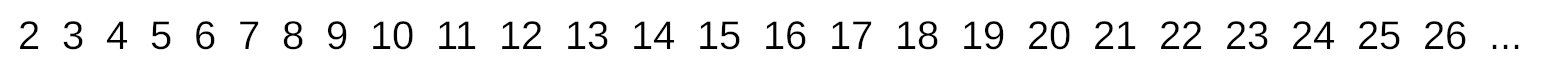
\includegraphics[width=\linewidth]{chapters/teorija-stevil/slike/reseto1}

Vemo, da je število $2$ praštevilo.
Večkratniki števila $2$ zato niso praštevila, ker so deljivi z $2$; torej jih
prečrtamo.

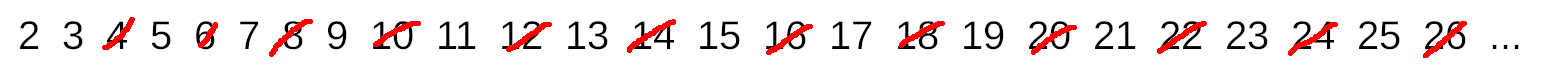
\includegraphics[width=\linewidth]{chapters/teorija-stevil/slike/reseto2}

Število $3$ je praštevilo, torej tudi večkratniki $3$ niso praštevila.

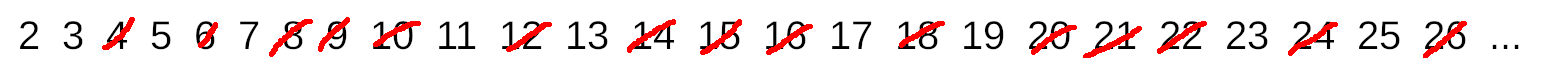
\includegraphics[width=\linewidth]{chapters/teorija-stevil/slike/reseto3}

Prišli so do števila $4$, ki je prečrtano, zato vemo, da ni praštevilo.
Ker je deljivo z $2$, smo vse večkratnike $4$ (ki so tudi večkratniki $2$), že
prečrtali, torej nam ni treba posebej črtati večkratnikov $4$.

Število $5$ je praštevilo (ker ni prečrtano), torej moremo prečrtati njegove
večkratnike.

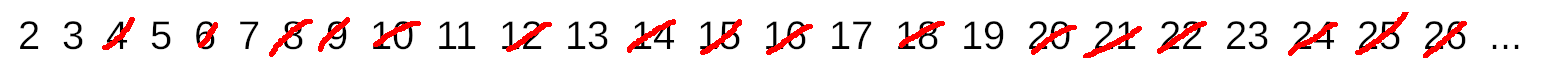
\includegraphics[width=\linewidth]{chapters/teorija-stevil/slike/reseto4}

Število $6$ je prečrtano, tako da ga preskočimo.

Postopek bi lahko nadaljevali, dokler ne pridemo do $26$ (oz.~do želene zgornje
meje), vendar nam ni treba.
Velja namreč naslednje; če je število $M$ produkt dveh števil, $M = A B$, potem
je vsaj eno od teh števil manjše od ali enako veliko kot $\sqrt{M}$.
Če bi bili obe števili večji kot $\sqrt{M}$, je njun produkt večji od $M$, to pa
ne mora veljati, ker je njun produkt ravno $M$.

V našem primeru smo torej lahko iskanje ustavili že pri $\sqrt{26}$, kar je
nekaj več kot $5$, zato moramo preveriti tudi $6$, več pa ne.

\begin{examples}
  Možna implementacija algoritma za iskanje praštevil je podana spodaj.
  Zapisana koda ohranja še dodatno informacijo; za vsako število si zapomnimo
  enega od njegovih praštevilskih deliteljev.
  %#insert python3 style.py < chapters/teorija-stevil/reseto.cpp
  Ta implementacija nam dovoljuje, da hitro poiščemo nekega delitelja poljubnega
  števila \verb+n+; preprosto pogledamo v \verb+reseto[n]+.
  Če najdemo \verb+0+, vemo, da je \verb+n+ praštevilo; sicer pa smo našli
  nekega delitelja.
\end{examples}

\chapter{Nekaj več o branju in pisanju}

\section{Scanf}

Funkcija \verb+scanf+ lahko bere različne vrste podatkov:
\begin{itemize}
	\item \verb+%s+ - beseda (vsi znaki razen praznih znakov (glej spodaj)) (\verb+char+)
	\item \verb+%c+ - en (poljuben) znak (\verb+char+)
	\item \verb+%d+ - število med $-2^{31}$ in $2^{31}-1$ (\verb+int+)
	\item \verb+%lld+ - število med $-2^{63}$ in $2^{63}-1$ (\verb+long long+)
	\item ...
\end{itemize}

\noindent Prazni znaki (whitespace) so znaki, ki jih ne vidimo:
\begin{itemize}
	\item \verb+\n+ nova vrstica
	\item \verb+\t+ zamik
	\item " " presledek
\end{itemize}

S formatnikom \verb+%s+ funkcija \verb+scanf+ bere do prvega takšnega znaka. Prebere tudi vse take znake, ki sledijo, a jih ne shrani. Naslednjič, ko jo pokličemo, bere od prvega nepraznega znaka naprej.

\begin{examples}

%#insert python3 style.py < chapters/inout_advanced/formatnik_s.cpp

\begin{inout}
Hello \\ \\ World!
\tcblower
Hello World!
\end{inout}


\end{examples}

\newpage
\section{Branje do konca vrstice}

Lahko določimo, da se \verb+scanf+ ne bo ustavil pri prvem praznem znaku, temveč šele pri koncu vrstice (ali kje drugje).

\begin{examples}

%#insert python3 style.py < chapters/inout_advanced/do_konca_vrstice.cpp

\begin{inout}
Beremo do konca vrstice.
\tcblower
Beremo do konca vrstice.
\end{inout}

\end{examples}

\verb+[...]+ - med oklepaje pišemo navodila, kakšne znake lahko bere
\begin{itemize}
	\item \verb+[a-z]+ - beri male črke angleške abecede
	\item \verb+[a-zA-Z0-9]+ - beri male in velike črke in številke
\end{itemize}

\verb+[^...]+ - beri vse do znakov, ki sledijo strešici
\begin{itemize}
	\item \verb+[^\n]+ - beri vse do \verb+\n+
\end{itemize}

%CHECK
\begin{errors}
Za razliko od \verb+%s+ funkcija \verb+scanf+ s \verb+[^\n]+ prebere vse do \verb+\n+, tega pa ne prebere in se ustavi pred njim. Ko funkcijo pokličemo naslednjič, začne tam, kjer je nazadnje ostala, kar je v tem primeru točno pred znakom \verb+\n+. Če jo torej ponovno pokličemo s parametrom \verb+[^\n]+, se ne bo nikamor premaknila, saj je pred njo znak za novo vrstico. \\
\end{errors}

%CHECK
\verb+%c+ - prebere en znak (\verb+char+), ki je lahko karkoli - črka, številka, prazen znak... \\
\verb+%*c+ - prebere en znak, a ga ne shrani \\
Funkcija \verb+getchar+ dela podobno, vzame en znak in ga ne shrani. \\

Za razliko od tega s formatnikom \verb+%s+ preberemo vse prazne znake med dvema
nepraznima nizoma in jih ne shranimo. Tudi, če bodo prazni znaki pred besedo,
jih bo program ignoriral in poiskal prvi neprazen znak.

\newpage
\section{Branje do konca vhoda}

Če vemo točno, koliko besed/številk/vrstic bomo imeli na vhodu, jih lahko preberemo s for zanko. Kako preberemo neznano količino podatkov na vhodu, tako da preberemo vse? \\
Če napišemo \verb+while(true)+ ali \verb+while(1)+, bomo sicer prebrali vse, a se program ne bo nikoli ustavil.
Namesto tega lahko napišemo:

\begin{examples}

%#insert python3 style.py < chapters/inout_advanced/do_konca_vhoda.cpp

\begin{inout}
1 2 3 4 5
\tcblower
1\\4\\9\\16\\25
\end{inout}
\end{examples}

\vskip 0.15in
%CHECK
\noindent Funkcija \verb+scanf+ vrne število formatnikov, ki jih je uspešno
prebrala (če ji kot parameter podamo samo \verb+%d+, bo vrnila $1$, če je
uspešno prebrala število, sicer pa 0). \verb+EOF+ (End of File) vrne, če na
vhodu ni ničesar več za prebrati. Tedaj se bo zanka ustavila. Če programu
vhodne podatke podajamo iz datoteke, se to zgodi avtomatsko ob koncu datoteke,
če pa mu podatke podajamo na roko, konec vhoda sporočimo s
\verb-Ctrl+D (Linux in MacOS)- ali \verb-Ctrl+Z- (Windows).

\begin{examples}

%#insert python3 style.py < chapters/inout_advanced/stevilo_prebranih.cpp

\begin{inout}
	5 8 100
	\tcblower
	3
\end{inout}
\begin{inout}
	5 8 miha
	\tcblower
	2
\end{inout}


\end{examples}

\newpage
\section{Branje in pisanje v in iz niza}

\verb+scanf+ uporabljamo za branje s standardnega vhoda, \verb+printf+ pa za pisanje na standardni izhod.
Namesto tega lahko beremo in pišemo tudi drugače, npr. v in iz nizov.
Za to uporabljamo funkciji \verb+sscanf+ in \verb+sprintf+, ki delata podobno kot \verb+scanf+ in \verb+printf+.

\begin{examples}

%#insert python3 style.py < chapters/inout_advanced/sprintf.cpp

\begin{inout}

\tcblower
a 157 Slovenska
\end{inout}

\end{examples}

\begin{errors}
Medtem ko \verb+%s+ praznih znakov ne shrani, jih \verb+%c+ obravnava tako kot
vse ostale. Če pogeldamo prejšnji primer vidimo, da je v funkciji
\verb+scanf+ pred \verb+%c+ presledek. Ker so med posameznimi podatki, ki
jih želimo prebrati, presledki, bi \verb+%c+ pobral presledek, ne pa črke,
ki mu sledi. Če med posamezne formatnike postavimo presledek, ta načeloma
pobere prazne znake do naslednjega drugačnega znaka, vendar to v splošnem
ni dobra praksa.
\end{errors}

\noindent Funkciji \verb+sscanf+ podamo tri parametre (ali več):
\begin{enumerate}
	\item ime niza, iz katerega naj bere
	\item tip podatka, ki naj ga prebere (niz, število...)
	\item kam naj ta podatek zapiše (ime spremenljivke)
\end{enumerate}
	
\noindent Funkciji \verb+sprintf+ prav tako podamo tri parametre (ali več):
\begin{enumerate}
	\item ime niza, kamor naj piše
	\item tip podatka, ki naj ga zapiše
	\item kaj naj zapiše (ime spremenljivke ali podatek sam)
\end{enumerate}

\newpage
\section{Branje in pisanje v in iz datoteke}

Podobno kot v niz lahko pišemo in beremo tudi v in iz datotek s funkcijama \verb+fscanf+ in \verb+fprintf+.

\begin{examples}

%#insert python3 style.py < chapters/inout_advanced/datoteke.cpp

\begin{inout}
{\color{blue} \bf in.txt:} \\
1 2 3 4 5 6 7
\tcblower
{\color{blue} \bf out.txt:} \\
1\\
4\\
9\\
16\\
25\\
36\\
49
\end{inout}

(Ta program ne bere s standardega vhoda in ne piše ne standardni izhod.)
\end{examples}

\verb+FILE+ - tip podatka
\verb+fopen+ - funkcija, s katero odpremo datoteko, podamo ji ime datoteke, ki
jo želimo odpreti in način \verb+"r"+ (\emph{read} - za branje) ali \verb+"w"+
(\emph{write} - za pisanje).\\ Datoteke, ki jih odpiramo za branje, morajo že
prej obstajati, sicer se bo program sesul. \\

Za datoteke, v katere pišemo, ni nujno, da že obstajajo. Če še ne obstajajo, bo
program ustvaril novo datoteko s tem imenom. Če že obstajajo, program ne bo
pisal na konec te datoteke, temveč bo pobrisal vso prejšnjo vsebino.
Če želimo obstoječi datoteki dodajati vsebino, moramo uporabiti način
\verb+"a"+ (\emph{append} - pripenjanje).

\verb+fclose+ - funkcija, ki zapre odprto datoteko, podamo ji ime datoteke

\chapter{Asimptotična notacija}

\section{Merjenje efektivnosti programa}

Pogosto obstaja več možnosti, kako se lahko lotimo reševanja danega problema.
Če želimo najti najmanjši element v seznamu, lahko pregledamo celoten seznam in
si beležimo najmanjšega, ki smo ga našli do sedaj, lahko pa celoten seznam
uredimo po vrsti in nato izberemo prvi element, na primer.
Pričakujemo lahko, da se bodo različni algoritmi za reševanje istega problema
razlikovali tudi po tem, kako hitro problem rešijo.
Kako pa v računalništvu izmerimo hitrost? Če delamo samo na enem računalniku,
lahko izmerimo, konkretno koliko časa je program potreboval, da je zaključil
z delovanjem. Na ta način lahko na primerih demonstriramo, da je nek algoritem
boljši od drugega; ko pa želimo naše rezultate deliti in primerjati z drugimi,
pa se ne moramo zanašati, da bodo imeli enako močen računalnik kot mi, in da
bodo njihovi testni primeri primerljivo zahtevni z našimi. Dejansko so težave
pri tem še hujše; na hitrost delovanja našega programa ne vpliva samo strojna
oprema računalnika (torej, kakšen procesor ima, koliko ima spomina itd.), temveč
tudi ostali programi, ki jih imamo hkrati odprte.
Če se želimo pogovarjati o hitrosti algoritmov, potrebujemo bolj abstraktno
orodje. Na pomoč pride asimptotična zahtevnost.

Da določimo hitrost našega programa, moramo prvo določiti, katere spremenljivke
vplivajo na čas delovanja, ter kako je čas od njih odvisen.
Rezultat take analize zapišemo kot izraz v oklepaje, pred katere zapišemo
veliko črko O: \(O(\ldots)\)
Poglejmo si primer.

%#insert python3 style.py < chapters/asimptoticna-notacija/poisci-najmanjsega.cpp

Funkcija \verb+poisci_najmanjsega+ sprejme število \(n\), ki pove dolžino seznama
\verb+arr+. Po seznamu se nato enkrat sprehodi, in si ob tem beleži indeks
najmanjšega elementa, ki ga je do sedaj našla.

Razmislimo, katere vse različne operacije program opravi.
\begin{itemize}
  \item 
	Večkrat med programom nastavimo neki spremenljivki novo vrednost.
  \item
	V vsaki iteraciji zanke prištejemo 1 spremenljivki \verb+i+.
  \item
	Poleg tega v vsaki iteraciji zanke tudi primerjamo \verb+i+ z \verb+n+,
  \item
	dvakrat dostopamo do nekega elementa v seznamu,
  \item
	ter ju primerjamo.
  \item
	Na koncu še enkrat dostopamo do elementa v seznamu, ter ga vrnemo.
\end{itemize}

Vse naštete operacije same po sebi \emph{trajajo} \(O(1)\) časa. To pomeni, da
se vedno izvajajo enako hitro, neodvisno od parametrov, ki jim podamo. Rečemo
tudi, da porabijo \emph{konstantno mnogo} časa.

Kolikokrat pa izvedemo te operacije? Analizirajmo najslabši primer za naš
program; če je seznam \verb+arr+ padajoče urejen. Tedaj bomo v vsaki iteraciji
zanke enkrat primerjali \verb+i < n+, dvakrat dostopali do elementov seznama,
enkrat primerjali \verb+arr[min_idx] > arr[i]+, enkrat nastavili \verb+min_idx+,
ter enkrat povečali \verb+i+. Zunaj zanke bomo nastavili \verb+min_idx+ ter
\verb+i+ na začetni vrednosti, ter še enkrat dostopali do elementa v seznamu.
Zanka se vedno izvaja za natanko \verb+n+ iteracij; vedno vsak element pregledamo
enkrat. Torej je celotna časovna zahtevnost našega programa \(O(3 + 6n)\).
Ker pa za velike \(n\) del zunaj zanke hitro postane nepomemben, ga ignoriramo.
Poleg tega ignoriramo tudi faktor pred členom \(n\) -- ker tako in tako ne moramo
vedeti, kako hitre so operacije v zanki v primerjavi druga z drugo, te konstante
ne moramo natančno določiti. Končna časovna zahtevnost našega programa je torej
\(O(n)\).

To je tudi najboljši možni algoritem za iskanje najmanjšega elementa v seznamu.
Če bi nek algoritem namreč deloval v hitrejšem času kot \(O(n)\), bi moral
nekatera mesta v seznamu izpustiti; če tedaj algoritmu podamo seznam, ki ima
najmanjši element ravno na takem mestu, ga algoritem ne bo našel, in bo podal
napačen odgovor.

Pomembna opazka je, da hitrost našega algoritma ni odvisna od velikosti števil
v seznamu, temveč le od velikosti seznama. Naslednji program prav tako poišče
najmanjše število v seznamu, vendar je konkretno počasnejši od zgornjega:

%#insert python3 style.py < chapters/asimptoticna-notacija/poisci-najmanjsega-slabsi.cpp

V tem programu imamo dve zanki; ena se sprehaja po vseh možnih vrednosti števil
v seznamu, druga pa preverja, če je ta element dejansko v seznamu. Vsakič, ko se
zunanja zanka izvede enkrat, se notranja izvede \verb+n+-krat (v najslabšem
primeru), zunanja zanka pa se izvede \verb|m+1|-krat. Torej je zahtevnost
\(O((m+1) \cdot n)\), oziroma \(O(mn + n)\). Člen \(n\) v vsoti pa je v vseh
primerih manjši od člena \(mn\) ali njemu enako velik, zato ga izpustimo.
Končna časovna zahtevnost drugega algoritma je torej \(O(mn)\).

\verb+int+ lahko hrani števila, velika do približno dve milijardi -- najslabšem
primeru je \(m\) torej približno \(2 \cdot 10^9\). Če prvi algoritem na nekem
računalniku potrebuje eno sekundo, da se konča, bi drugi algoritem v najslabšem
primeru na istem računalniku potreboval več kot šestdeset let.

\begin{examples}

  Naslednji program za vsako število v seznamu \verb+arr+ poišče število števil desno od njega, ki so večja.

  %#insert python3 style.py < chapters/asimptoticna-notacija/stevilo-vecjih.cpp

  Notranja zanka se v prvi iteraciji izvede \((n-1)\)-krat, v drugi iteraciji
  \((n-2)\)-krat, v tretji \((n-3)\)-krat, itd. V zadnji iteraciji se sploh ne
  izvede. Skupaj se koda znotraj druge zanke torej izvede
  \((n-1) + (n-2) + \ldots + 1 + 0 = \frac{n(n-1)}{2}\)-krat. Spet ignoriramo
  konstanto \(\frac{1}{2}\) ter člen samo z \(n\), in pridemo do zahtevnosti
  \(O(n^2)\).

\end{examples}

\begin{examples}

  Naslednji program preveri, če je število \(n\) praštevilo.

  % Zahvala Roku Lavriču za popravek v kodi
  %#insert python3 style.py < chapters/asimptoticna-notacija/prastevilo.cpp

  Program ima eno zanko, ki se sprehaja toliko časa, da kvadrat spremenljivke
  \(i\) postane večji kot \(n\), oz.~dokler je \(i \le \sqrt{n}\). Zanka se torej
  izvede v \(O(\sqrt{n})\).

\end{examples}

\newpage
\section{Klasifikacija}

Računalnik lahko v eni sekundi opravi približno \(10^7\) operacij. Da določimo,
kako dober algoritem potrebujemo za rešitev neke naloge, lahko preverimo
omejitve vhodnih podatkov. Spodnja tabela prikazuje nekaj pogostih časovnih
zahtevnosti, ter pripadajoče največje omejitve. Z uporabo te tabele lahko
vnaprej določimo, kakšno največjo časovno zahtevnost mora imeti naš program,
da reši določeno nalogo.

\begin{table}[h!]
  \centering
  \begin{tabular}{|c|c|c|}
	\hline
	Zahtevnost & Omejitev za \(n\) & Ime zahtevnosti \\
	\hline
	\(O(1)\) & brez & \emph{konstantna} \\
	\(O(\log n)\) & zelo visoka & \emph{logaritemska} \\
	\(O(\sqrt{n})\) & \(10^{14}\) & \emph{korenska} \\
	\(O(n)\) & \(10^7\) & \emph{linearna} \\
	\(O(n \log n)\) & \(10^6\) & \\
	\(O(n^2)\) & \(10^4\) & \emph{kvadratna} \\
	\(O(n^3)\) & \(300\) & \emph{kubična} \\
	\(O(2^n)\) & \(20\) & \emph{eksponentna} \\
	\hline
  \end{tabular}
\end{table}

\chapter{Urejanje}

\section{Osnovno o urejanju}

V programih pogosto želimo nek seznam števil urediti po vrsti.
V ta namen lahko napišemo svojo funkcijo, ki implementira enega od znanih
algoritmov za urejanje; npr.~\textit{bubble sort}, \textit{insertion sort},
\textit{quick sort}, ipd. Ker pa so učinkovite implementacije pogosto komplicirane
in se pri pisanju hitro zmotimo, je bolje, da uporabimo funkcije, ravno v ta
namen vključene v standardno knjižnjico. Za to bomo potrebovali na začetek
programa dodati še dve vrstici:

%#insert python3 style.py < chapters/urejanje/algorithm.cpp

Ukaz \verb+#include+ že poznamo, opazimo pa, da tokrat za spremembo nima končnice
\verb+.h+. To je zato, ker funkcije, ki smo jih uporabljali do sedaj, izvirajo
iz jezika C, tokrat pa potrebujemo funkcijo, napisano posebaj za C++. To razloži
tudi drugo vrstico; vse funkcije v standardni knjižnjici v C++ so vključene
v imenski prostor \verb+std+. Če jih želimo klicati, moramo pred ime funkcije
vedno napisati \verb+std::+, ali pa na začetek programa vključiti vrstico
\verb+using namespace std+.

Sedaj lahko uporabimo funkcijo \verb+sort+, ki sprejme dva argumenta;
začetek in konec predela spomina, ki ga želimo urediti. Poglejmo si enostavni
primer.

%#insert python3 style.py < chapters/urejanje/uporaba.cpp


Program prebere število \(n\), za njim pa še \(n\) števil, jih uredi naraščajoče,
in jih izpiše. Funkcijo \verb+sort+ smo poklicali tako, da smo kot prvi argument
podali seznam \verb+arr+, kot drugi argument pa konec predela seznama, ki ga
želimo urediti; to zapišemo kot \verb|arr+n|. Točen pomen tega izraza bomo
spoznali v prihodnje, za sedaj pa bomo kot drugi argument vedno podali seznam
plus njegovo dolžino.

Optimalna časovna zahtevnost algoritma za urejanje je \(O(n \log n)\). To v praksi
pomeni, da bo urejanje delovalo dovolj hitro za \(n \le 10^6\). Če imamo več
podatkov kot toliko, bo urejaje trajalo predolgo in naša rešitev ne bo sprejeta.

\section{Primerjalna funkcija}

Če želimo urediti seznam padajoče namesto naraščajoče, lahko seznam prvo uredimo
naraščajoče, in ga nato obrnemo. Ker s tem dobimo veliko dodatnega dela, je
bolje, da funkciji \verb+sort+ podamo lastno primerjalno funkcijo. Le-ta mora
sprejeti dva argumenta ter vrniti \verb+bool+, in sicer; če mora biti prvi
argument v urejenem seznamu levo od drugega, mora funkcija vrniti \verb+true+,
sicer pa \verb+false+.

Če ne podamo tretjega argumenta, se \verb+sort+ obnaša tako, kot da bi podali
naslednjo funkcijo:

%#insert python3 style.py < chapters/urejanje/compare.cpp

Če želimo urediti seznam padajoče, moramo le podati nasprotno funkcijo:

%#insert python3 style.py < chapters/urejanje/nasprotno.cpp

\subsection{Urejanje sestavljenih podatkov}

Recimo, da imamo v nalogi dana imena tekmovalcev ter točke, ki so jih ti
tekmovalci dosegli na tekmovanju, naš cilj pa je, da izpišemo imena tekmovalcev
po vrsti glede na doseženo število točk. Če bomo prebrali točke in imena v
različna seznama, ter uredili seznam točk, bo seznam imen ostal nespremenjen in
ne bomo več vedeli, katero ime pripada katerim točkam.

Kako uredimo oba seznama hkrati? Bolj enostavna možnost je uporaba \verb+struct+,
ki pa ga še ne poznamo. Namesto tega si lahko pripravimo seznam indeksov, ki
na začetku na \verb+i+-tem mestu hrani številko \verb+i+. Če sestavimo funkcijo
\verb+compare+ tako, da sprejme dva indeksa, ter ju uredi glede na vrednosti
v tabeli s točkami na pripadajočih indeksih. Urejamo pa ne tabele s točkami,
temveč novo tabelo indeksov.
Na ta način se tabeli s točkami in z imeni ne bosta spreminjali,
in bodo točke pripadale imenu na istem indeksu.

\begin{examples}

Primer implementacije opisane rešitve:

%#insert python3 style.py < chapters/urejanje/kombinirani.cpp

\begin{inout}
  5 \\
  France 37 \\
  Gregor 34 \\
  Julija 38 \\
  Matija 29 \\
  Urska 8 \\
  \tcblower
  Julija
  France
  Gregor
  Matija
  Urska
\end{inout}

\end{examples}

\chapter{Spomin in kazalci}

\section{Računalniški spomin}

Spomin, pomnilnik ali angl.~RAM (\textit{Random access memory})
je ključna komponenta v računalniku. Med tekom programa so v njem vse
spremenljivke, ki jih program uporablja. S spremenljivkami lahko naredimo tudi
več, kot smo se do sedaj naučili, vendar pa moramo za to razumeti, kako je
spomin zgrajen.

Osnovna enota za merjenje količine informacij je \emph{bit}.
En bit informacij ustreza odgovoru na eno vprašanje tipa da ali ne
-- če nam nekdo pove, da so vrata zaprta, nam je podal en bit informacij,
ker so lahko vrata bodisi odprta bodisi zaprta.
Če imamo v omari dva para hlač, dve majici in dve kapi, lahko opišemo,
kako smo oblečeni, s tremi biti informacije -- za vsak kos oblačila porabimo
en bit.

V računalništvu bite najpogosteje označujemo z ničlami in enicami.
Običajno ničla predstavlja odgovor ``ne'' na dano vprašanje,
enica pa odgovor ``da''. Bit pa je zelo majhna količina informacije, zato
pogosto govorimo v večjih enotah, kot so \emph{bajti}, \emph{kilobajti},
\emph{megabajti} itd. En bajt ustreza osmim bitom, kilobajt je tisoč bajtov,
megabajt je tisoč kilobajtov, gigabajt je tisoč megabajtov, in terabajt je
tisoč gigabajtov.

\begin{errors}
  Pogosto, a napačno mišljenje je, da kilobajt ustreza 1024 bajtom.
  Ta mit izvira iz zgodnjih časov računalništva, ko so za hitrejše
  računanje nekateri programi med spominskimi enotami pretvarjali
  s to napačno številko; 1024 je namreč potenca 2, s katerimi računalniki
  pogosto lahko hitreje računajo.
  Če za pretvorbo uporabljamo faktor 1024, moramo za enote podati
  \emph{kibibajte} (KiB), \emph{mebibajte} (MiB), \emph{gibibajte} (GiB),~ipd.,
  namesto običajnih SI predpon.
\end{errors}

Računalniški spomin je sestavljen iz spominskih celic, ki so dolge en bajt.
Vsaka od teh celic ima svoj \emph{naslov} -- številko, s katero lahko to
celico ločimo od ostalih. Naslovi so zaporedne številke od 0 do velikosti
pomnilnika, ki ga imamo nameščenega v računalniku.
Celice so naraščajoče urejene po svojih naslovih -- celica številka 150337 je
sosednja celicama s številkama 150336 in 150338.

Upravljanje z računalniškim spominom je ena od nalog operacijskega sistema.
Naši programi operacijski sistem med izvajanjem prosijo za neko količino spomina,
operacijski sistem pa določi, katere spominske celice bo program prejel.
Te celice tedaj pripadajo programu, dokler se ta ne zaključi, ali dokler tega
spomina ne vrne operacijskemu sistemu na drugačen način. Med izvajanjem
našega programa praviloma noben drug program nima dostopa do tega dela
spomina.

Kako pa program ve, koliko spomina bo potreboval? Da to izračuna, se zanaša
na tipe. Vsaka spremenljivka ima tip, vsak tip pa ima fiksno dolžino, ki jo
zavzame v spominu. Dolžine pogostih tipov so sledeče:
\begin{itemize}
  \item \verb+int+: 4 bajti
  \item \verb+long long+: 8 bajtov
  \item \verb+char+: 1 bajt
  \item \verb+bool+: 1 bajt
\end{itemize}
Spremenljivke, ki v spominu zavzamejo več kot 1 bajt, moramo shraniti v več
kot eno spominsko celico. Celice, v katere te vrednosti zapišemo, so v spominu
zaporedne; če imamo spremenljivko tipa \verb+int+, bo zavzela 4 zaporedne celice.

\section{Kazalci}

\begin{errors}
  Kazalci so pomemben koncept v programiranju, in razumevanje kazalcev je ključno
  za razumevanje bolj zapletenih podatkovnih struktur ter nekaterih algoritmov.
  S kazalci pa se lahko zelo hitro zmotimo, in razhroščevanje kode z veliko
  kazalci je pogosto zelo zapleteno. Zaradi tega in drugih razlogov
  se kazalcem izogibamo v tekmovalnem programiranju, razen če jih res nujno
  potrebujemo.
\end{errors}

Ker so spominski naslovi številke, jih lahko shranjujemo, kakor shranjujemo
ostale številke; za to pa imamo v C++ na voljo poseben tip, ki mu rečemo
\emph{kazalec} (angl.~\textit{pointer}).
Pravzaprav kazalec ni sam svoj tip, ampak razširitev nekega drugega tipa;
pravimo, da kazalec \emph{kaže na drug tip}.
Da ustvarimo nov kazalec, zapišemo ime tipa, na katerega želimo kazati,
nato pa pred ime spremenljivke damo zvezdico~\verb+*+.
Kazalcu lahko nastavimo vrednost tako, da vanj shranimo naslov neke
spremenljivke, ki smo že ustvarili. Do naslova dostopamo z operatorjem~\verb+&+.
Da dostopamo do vrednosti, shranjene v celici, na katero kazalec kaže,
uporabimo operator \verb+*+ (ki ima drugačen pomen, kot zvezdica v deklaraciji
spremenljivke).

\begin{examples}
  %#insert python3 style.py < chapters/kazalci/sintaksa.cpp
\end{examples}

Vse, kar smo sedaj delali s kazalci, je bilo možno (in lažje) narediti tudi z
običajnimi spremenljivkami. Kazalci, ki kažejo na spremenljivke, ki tako in tako
že obstajajo, so bolj ali manj neuporabni. Kako pa naredimo kazalec, ki kaže
na del spomina, v katerem ni nobene spremenljivke?

Če želimo storiti kaj takega, moramo prevzeti odgovornost za upravljanje spomina
v našem programu. Do sedaj je za to skrbel prevajalnik, ki je v naš program na
pravilna mesta zapisal ukaze, ki si spomin sposojajo od operacijskega sistema,
ter ga vračajo, ko ga ne potrebujemo več. Bolj natančno; ko smo deklarirali
spremenljivko, je prevajalnik poskrbel, da prosimo za natanko toliko spomina,
kolikor ga za to spremenljivko potrebujemo (zato moramo za vsako spremenljivko
zapisati tip), ter si njegov naslov zapomnil,
ko pa spremenljivke nismo več potrebovali, je prevajalnik poskrbel, da ta del
spomina vrnemo operacijskemu sistemu; temu pravimo \emph{sprostitev}
(angl.~\textit{deallocation}).

Za bolj sofisticirano uporabo spomina moramo ti vlogi prevzeti mi. Za to sta
nam na voljo dve funkciji: \verb+malloc+ in \verb+free+. Da ju uporabljamo,
moramo vključiti \verb+stdlib.h+.
Oblika funkcij je naslednja:
%#insert python3 style.py < chapters/kazalci/opis_malloc_free.cpp
V obliki je posebnost, ki je še nismo omenili; ni namreč nujno, da ima vsak
kazalec tip. Lahko imamo kazalce, ki kažejo na del spomina, mi pa (še) ne vemo,
kaj je v tistem delu spomina shranjeno. Za take kazalce pravimo, da kažejo
na \verb+void+, kar pa ne pomeni, da ne kažejo na nič; na lokaciji v spominu,
kamor kažejo, je nekaj shranjeno; mi samo ne vemo, kako naj te podatke
interpretiramo.

Funkcija \verb+malloc+ sprejme en argument, in vrne kazalec na \verb+void+.
Ta argument je tipa \verb+size_t+, ki je za naše potrebe skoraj enak tipu
\verb+unsigned long long+; to je torej številka. Pove, koliko bajtov spomina si
želimo sposoditi od operacijskega sistema. \verb+malloc+ nato vrne kazalec na
prvi naslov znotraj bloka spomina, ki smo si ga ravno sposodili. Ker operacijski
sistem ne ve, kaj bomo v ta spomin shranili, nam \verb+malloc+ vrne \verb+void*+,
mi pa ga moramo pretvoriti v pravi tip kazalca. To storimo tako, da tik pred
klic funkcije v oklepaje zapišemo želeni tip kazalca.

Funkcija \verb+free+ je ravno nasprotna od \verb+malloc+; sprejme kazalec, ki ga
nam je dal \verb+malloc+, ter sprosti del spomina, na katerega kazalec kaže.
Kazalec bo po klicu \verb+free+ še vedno obstajal, in bo še vedno kazal na isto
mesto. Edina sprememba je, da del spomina, na katerega kaže, ne pripada več
našemu programu, in ga ne smemo uporabljati.

\begin{examples}
  %#insert python3 style.py < chapters/kazalci/dynamic_memory_management.cpp
  Operator \verb+sizeof+ lahko uporabljamo, da si pomagamo pri določevanju
  velikosti tipov.
\end{examples}

\newpage
\section{Kako delujejo seznami}

Nič nas ne omejuje, da od operacijskega sistema zahtevamo zelo velik blok
spomina, tudi po več sto tisoč bajtov. Pa imamo lahko kakšen utemeljen razlog,
da si toliko spomina izposodimo? Da, ravno to stori prevajalnik, ko ustvarimo
seznam. Poglejmo si, kako ustvarimo seznam samo s kazalci.

\begin{examples}
  %#insert python3 style.py < chapters/kazalci/seznam.cpp
\end{examples}

V zgornjem primeru uporabljamo dva nova operatorja na kazalcih; seštevanje in
oglate oklepaje. Če kazalcu \verb+seznam+ prištejemo število \verb+i+, dobimo
nov kazalec, ki kaže na mesto \verb|seznam + (velikost tipa) * i|, torej na
idealno mesto, kamor zapišemo \verb+i+-ti element seznama, če jih zapisujemo
enega za drugega.

Drug novi operator so oglati oklepaji -- ti se obnašajo popolnoma enako kot
v seznamih. Oglati oklepaj \verb+seznam[i]+ je pravzaprav krajšava za zapis
\verb|*(seznam+i)|, torej za dostop do \verb+i+-tega elementa v bloku spomina.

Tudi seznami, kakor smo jih spoznali prej, so dejansko kazalci na blok spomina,
le da s tem spominom upravlja prevajalnik. Trik s prištevanjem števila k
kazalcu deluje tudi za prištevanje števila k seznamu.

\section{Podajanje po referenci}

Opazimo, da smo operator \verb+&+ že srečali, in sicer čisto na začetku.
Pri branju številk iz vhoda moramo v \verb+scanf+ zapisati ta operator pred
imenom spremenljivke. Sedaj razumemo, zakaj je temu tako; \verb+scanf+ sprejme
kazalce na spremenljivke, ki jih želimo prebrati, ter popravi vrednosti, na
katere kažejo kazalci, s prebranimi vrednostmi.

\begin{examples}
  \verb+scanf+ je tudi funkcija, le da je nismo zapisali mi.
  Zmožna pa je nečesa, česar naše funkcije niso sposobne; spremeniti vrednosti
  spremenljivk zunaj nje. Spodnji program se ne bo niti prevedel:

  %#insert python3 style.py < chapters/kazalci/lokalne_spremenljivke.cpp

  Naslednji program pa se bo prevedel, vendar bo morda izhod v nasprotju s
  pričakovanji:

  %#insert python3 style.py < chapters/kazalci/lokalne_spremenljivke_2.cpp

  \begin{inout}
	\tcblower
	3
  \end{inout}
\end{examples}

Spremenljivke, ki jih deklariramo v funkciji, to je znotraj telesa funkcije,
ali pa v seznamu argumentov, so lokalne na to funkcijo -- zunaj nje sploh ne
obstajajo. Če želimo, da funkcija popravi neko vrednost, ki jo uporabljamo tudi
zunaj funkcije, smo do sedaj lahko to naredili samo tako, da smo spremenljivko
naredili globalno -- torej dostopno vsem funkcijam
(tudi \verb+main+ je funkcija). Kaj pa, če želimo neko spremenljivko na tak
način deliti samo med dvema funkcijama?

Da odgovorimo na to vprašanje, moramo razumeti, kako se argumenti podajajo v
funkcije. Ko neko funkcijo pokličemo, se argumenti, ki jih funkciji podamo,
\emph{prekopirajo} v poseben del spomina, ki ji pripada. Ko smo znotraj ene
funkcije, ne poznamo imena spremenljivk v drugih funkcijah; prav tako ne vemo,
kje so te spremenljivke shranjene. Nič pa nam ne preprečuje, da spreminjamo
spomin, ki našemu programu pripada, pa četudi je zunaj funkcije;
razen tega, da ne vemo, kateri del spomina je naš, in kateri ni.
Lahko si predstavljamo, da smo zabredli v spominsko džunglo, v kateri
ne prepoznamo prave poti do spremenljivk, ki jih želimo popraviti. Če pa s seboj
prinesemo zemljevid, bomo nenadoma to lahko naredili. Ta zemljevid je kazalec.

Funkcija lahko brez težav sprejme kazalec kot argument. Če to storimo, pravimo,
da smo spremenljivki vrednost podali \emph{po referenci}
(angl.~\textit{pass by reference}), namesto da bi argument podali običajno,
čemur pravimo \emph{podajanje po vrednosti} (angl.~\textit{pass by value}).
Kazalec, ki smo ga podali, se bo še vedno prekopiral v del spomina, ki pripada
funkciji; vrednost, na katerega kazalec kaže, pa bo ostala tam, kjer je.
Tako lahko skozi kazalec spremenimo vrednosti spremenljivk zunaj funkcije.

\begin{examples}
  Primera od zgoraj, narejena tako, da delujeta.

  %#insert python3 style.py < chapters/kazalci/pass_by_reference.cpp

  Kot vidimo, mora funkcija vedno sprejeti tudi argument, ki ga spremeni.

  %#insert python3 style.py < chapters/kazalci/pass_by_reference_2.cpp

\end{examples}

\end{document}